% ============================================================
%  RL Dynamic Control of a CO2-to-Methanol Plant
%  Technical Report -- extension of the EURECHA project
% ============================================================
\documentclass[11pt,a4paper]{article}

\usepackage[utf8]{inputenc}
\usepackage[T1]{fontenc}
\usepackage{lmodern}
\usepackage[margin=2.4cm]{geometry}
\usepackage{graphicx}
\usepackage{booktabs}
\usepackage{amsmath,amssymb}
\usepackage{xcolor}
\usepackage{hyperref}
\usepackage{caption}
\usepackage{subcaption}
\usepackage{float}
\usepackage{enumitem}
\usepackage{tabularx}
\usepackage{fancyhdr}

\definecolor{accentblue}{HTML}{264653}
\definecolor{accentteal}{HTML}{2A9D8F}
\definecolor{accentred}{HTML}{E63946}
\definecolor{lightgrey}{HTML}{F5F5F5}

\hypersetup{
  colorlinks=true,
  linkcolor=accentblue,
  citecolor=accentblue,
  urlcolor=accentteal,
}

\pagestyle{fancy}
\fancyhf{}
\fancyhead[L]{\small\textcolor{gray}{RL Dynamic Control -- EURECHA extension}}
\fancyhead[R]{\small\textcolor{gray}{\thepage}}
\renewcommand{\headrulewidth}{0.4pt}

\title{%
  \vspace{-1.5cm}
  \textbf{Reinforcement Learning for Dynamic Operation\\
  of a CO\textsubscript{2}-to-Methanol Plant}\\[6pt]
  \large Technical Report -- extension of the EURECHA Process Design Contest
}
\author{Jose Ma.\ Contreras P.}
\date{\today}

\begin{document}
\maketitle
\thispagestyle{fancy}

% ============================================================
\begin{abstract}
\noindent
This report studies whether reinforcement learning can operate a
cement-integrated CO\textsubscript{2}-to-methanol plant profitably under
volatile electricity prices. A Gymnasium environment couples hourly plant
dynamics, economic rewards, GB/NL electricity-price traces, and Gaussian
Process surrogate models derived from the Aspen-calibrated EURECHA base case.
Soft Actor-Critic (SAC) is the strongest algorithm in the tested setup:
under the internally consistent corrected v2 surrogate evaluation it achieves
\textbf{2915.6} scaled \pounds/week on GB prices, a \textbf{+487\%} improvement
over constant full-load operation, with 0\% GPR extrapolation warnings.
Cross-market transfer is promising: a GB-trained SAC evaluated on NL prices
retains essentially the same original-v1 reward (3227 to 3222), although those
absolute transfer values inherit the v1 extrapolation caveat.

The central limitation is surrogate trustworthiness. The original SAC policy
triggered GPR extrapolation warnings on 96.1\% of GB evaluation steps. A v2
pseudo-labelled surrogate correction removes that warning and preserves large
RL value, but it has not been checked against Aspen in the low-load region. A v3 refit
extends $F_{\mathrm{H}_2}$ coverage and fits cleanly ($R^2_{\mathrm{LCOM}} =
0.99981$), yet the v2-trained Fix~(c) policy becomes uneconomic when scored on
v3 ($-161.6 \pm 6.4$), showing that fresh SAC retraining and Aspen low-load
validation are still required. A flowsheet GNN extension is useful when
reframed as per-edge physical-state prediction ($R^2 = 0.997$ across 104
outputs), not as direct graph-level LCOM prediction. PPO fixes, GNN confidence
penalties, and the Pareto sweeps are kept as concise negative results.
\end{abstract}

\vspace{0.3cm}

% ============================================================
\section{Introduction}

The parent EURECHA project designs a large-scale CO\textsubscript{2}-to-methanol
process co-located with a cement kiln. Fresh CO\textsubscript{2}
(899~kmol/hr) is hydrogenated with green H\textsubscript{2} from a 270~MW
PEM electrolyser. A recycle loop with purge achieves high overall conversion,
producing approximately 213~kt/yr of methanol. The steady-state design and
economic model are Aspen-calibrated at the base case and then represented by
low-dimensional surrogate models for optimisation.

This extension asks a dynamic operating question: can an RL controller exploit
hourly electricity-price volatility by changing electrolyser load and reactor
conditions, instead of running the plant at constant full load? That question
is economically important because electricity dominates variable cost for
green methanol, and volatile day-ahead prices create hours where hydrogen
production is either attractive or damaging.

The answer depends on two things. First, the policy must actually learn a
profitable dispatch strategy. Second, the surrogate models used to score that
strategy must be trustworthy in the operating region discovered by the agent.
The main scientific story is therefore not simply ``SAC wins''. It is:
\emph{SAC can learn high-value dynamic operation, but surrogate coverage and
pending Aspen validation are the limiting evidence gap.}

% ============================================================
\section{Methods}

\subsection{Gymnasium Environment}

The environment is an hourly-step Gymnasium model with an 8-dimensional
observation vector: electricity price, electrolyser load, H\textsubscript{2}
buffer level, reactor temperature, reactor pressure, methanol rate, hour of
day, and day of week. The continuous action vector sets electrolyser load,
reactor temperature, and reactor pressure. First-order lags
($\tau_{\mathrm{load}}=0.3$, $\tau_T=0.5$, $\tau_P=0.7$~hr) give the plant
inertia rather than letting actions jump the process state instantly.

\subsection{Reward Function}

The base reward is a scaled hourly economic profit:
\begin{align}
  R = 10^{-3}\big(&
      \text{MeOH revenue}
      + \text{CO}_2\text{ credits}
      - \text{electricity cost} \nonumber\\
      &{} - \text{utility cost}
      - \text{ramp penalty}
      - \text{constraint penalties}\big).
\end{align}
Economic constants are single-sourced from the EURECHA project: e-methanol
\pounds800/t, CO\textsubscript{2} credits \pounds80/t, 50~kWh/kg
H\textsubscript{2} electrolyser specific power, and the Aspen heat-integration
utility basis.

\subsection{Surrogate Modelling}

Four evidence tiers are kept separate throughout the report:
\begin{enumerate}[nosep]
  \item \textbf{Aspen-calibrated base case:} the original EURECHA steady-state
        process design and economics.
  \item \textbf{Pseudo-labelled surrogate extensions:} v2 and v3 GPRs fitted
        to the simplified process model, not to new Aspen runs.
  \item \textbf{Corrected surrogate evaluation:} SAC policies evaluated on
        internally consistent v2/v3 surrogate surfaces with explicit
        extrapolation monitoring.
  \item \textbf{Pending Aspen validation:} 20 low-load validation points have
        been generated but not yet run in Aspen Plus.
\end{enumerate}

The original v1 GPRs are trained on a 500-point Latin Hypercube sample from
the simplified process model around the Aspen-calibrated design envelope.
The v2 correction augments that set with pseudo-labelled points in the SAC
operating region. The v3 correction extends the LCOM/utility
$F_{\mathrm{H}_2}$ domain to [800, 3200]~kmol/hr and is evaluated as a
follow-up pseudo-labelled surface, not as an Aspen-labelled surface.

\subsection{Agents and Baselines}

Three agents are tested: SAC, PPO, and tabular Q-learning. SAC and PPO use
Stable-Baselines3 continuous-control policies; Q-learning uses a
$10\times5\times5$ discretised action grid. Baselines are constant full-load
operation at nominal reactor conditions and a price-threshold rule that
reduces load during high-price hours.

% ============================================================
\section{Base RL Results}

Table~\ref{tab:base-corrected} is the most important RL result because it
places the original v1 performance beside the corrected v2 evaluation. The
original SAC reward is high, but it is not a defensible standalone profit estimate: it
triggers extrapolation warnings on 96.1\% of GB evaluation steps. The current
best internally consistent corrected v2 policy is Fix~(c), the v2 surrogate
plus variance-penalty SAC.

\begin{table}[H]
  \centering
  \caption{GB evaluation summary from available outputs. Rewards are scaled
           \pounds/week. v1 rows are useful for algorithm ranking but carry
           the GPR-extrapolation caveat; Fix~(c) is the corrected v2 result.}
  \label{tab:base-corrected}
  \small
  \begin{tabular}{l rrrr}
    \toprule
    \textbf{Policy} & \textbf{Reward} & \textbf{Std}
      & \textbf{CO\textsubscript{2} util.} & \textbf{GPR extrap.} \\
    \midrule
    Full-load baseline       & 496.7  & 821.2 & 0.938 & 0.0\% \\
    Rule-based threshold     & 1764.9 & 177.2 & 0.943 & 0.0\% \\
    Original PPO (v1)        & 1710.2 & 425.1 & 0.935 & 97.0\% \\
    Q-learning (v1)          & 2700.5 & 214.7 & 0.935 & 37.2\% \\
    Original SAC (v1)        & 3194.4 & 52.1  & 0.935 & 96.1\% \\
    Fix~(c) SAC (v2 + pen.)  & \textbf{2915.6} & \textbf{35.8} & 0.848 & \textbf{0.0\%} \\
    \bottomrule
  \end{tabular}
\end{table}

The corrected v2 result is still large: Fix~(c) improves on constant
full-load by +487\% and on the rule-based threshold by about 65\%. This is
the defensible dynamic-dispatch contribution. SAC is also the strongest
algorithm in the tested setup, while PPO is retained mainly as a collapsed
algorithmic baseline and Q-learning as a coarse but informative comparison.

\begin{figure}[H]
  \centering
  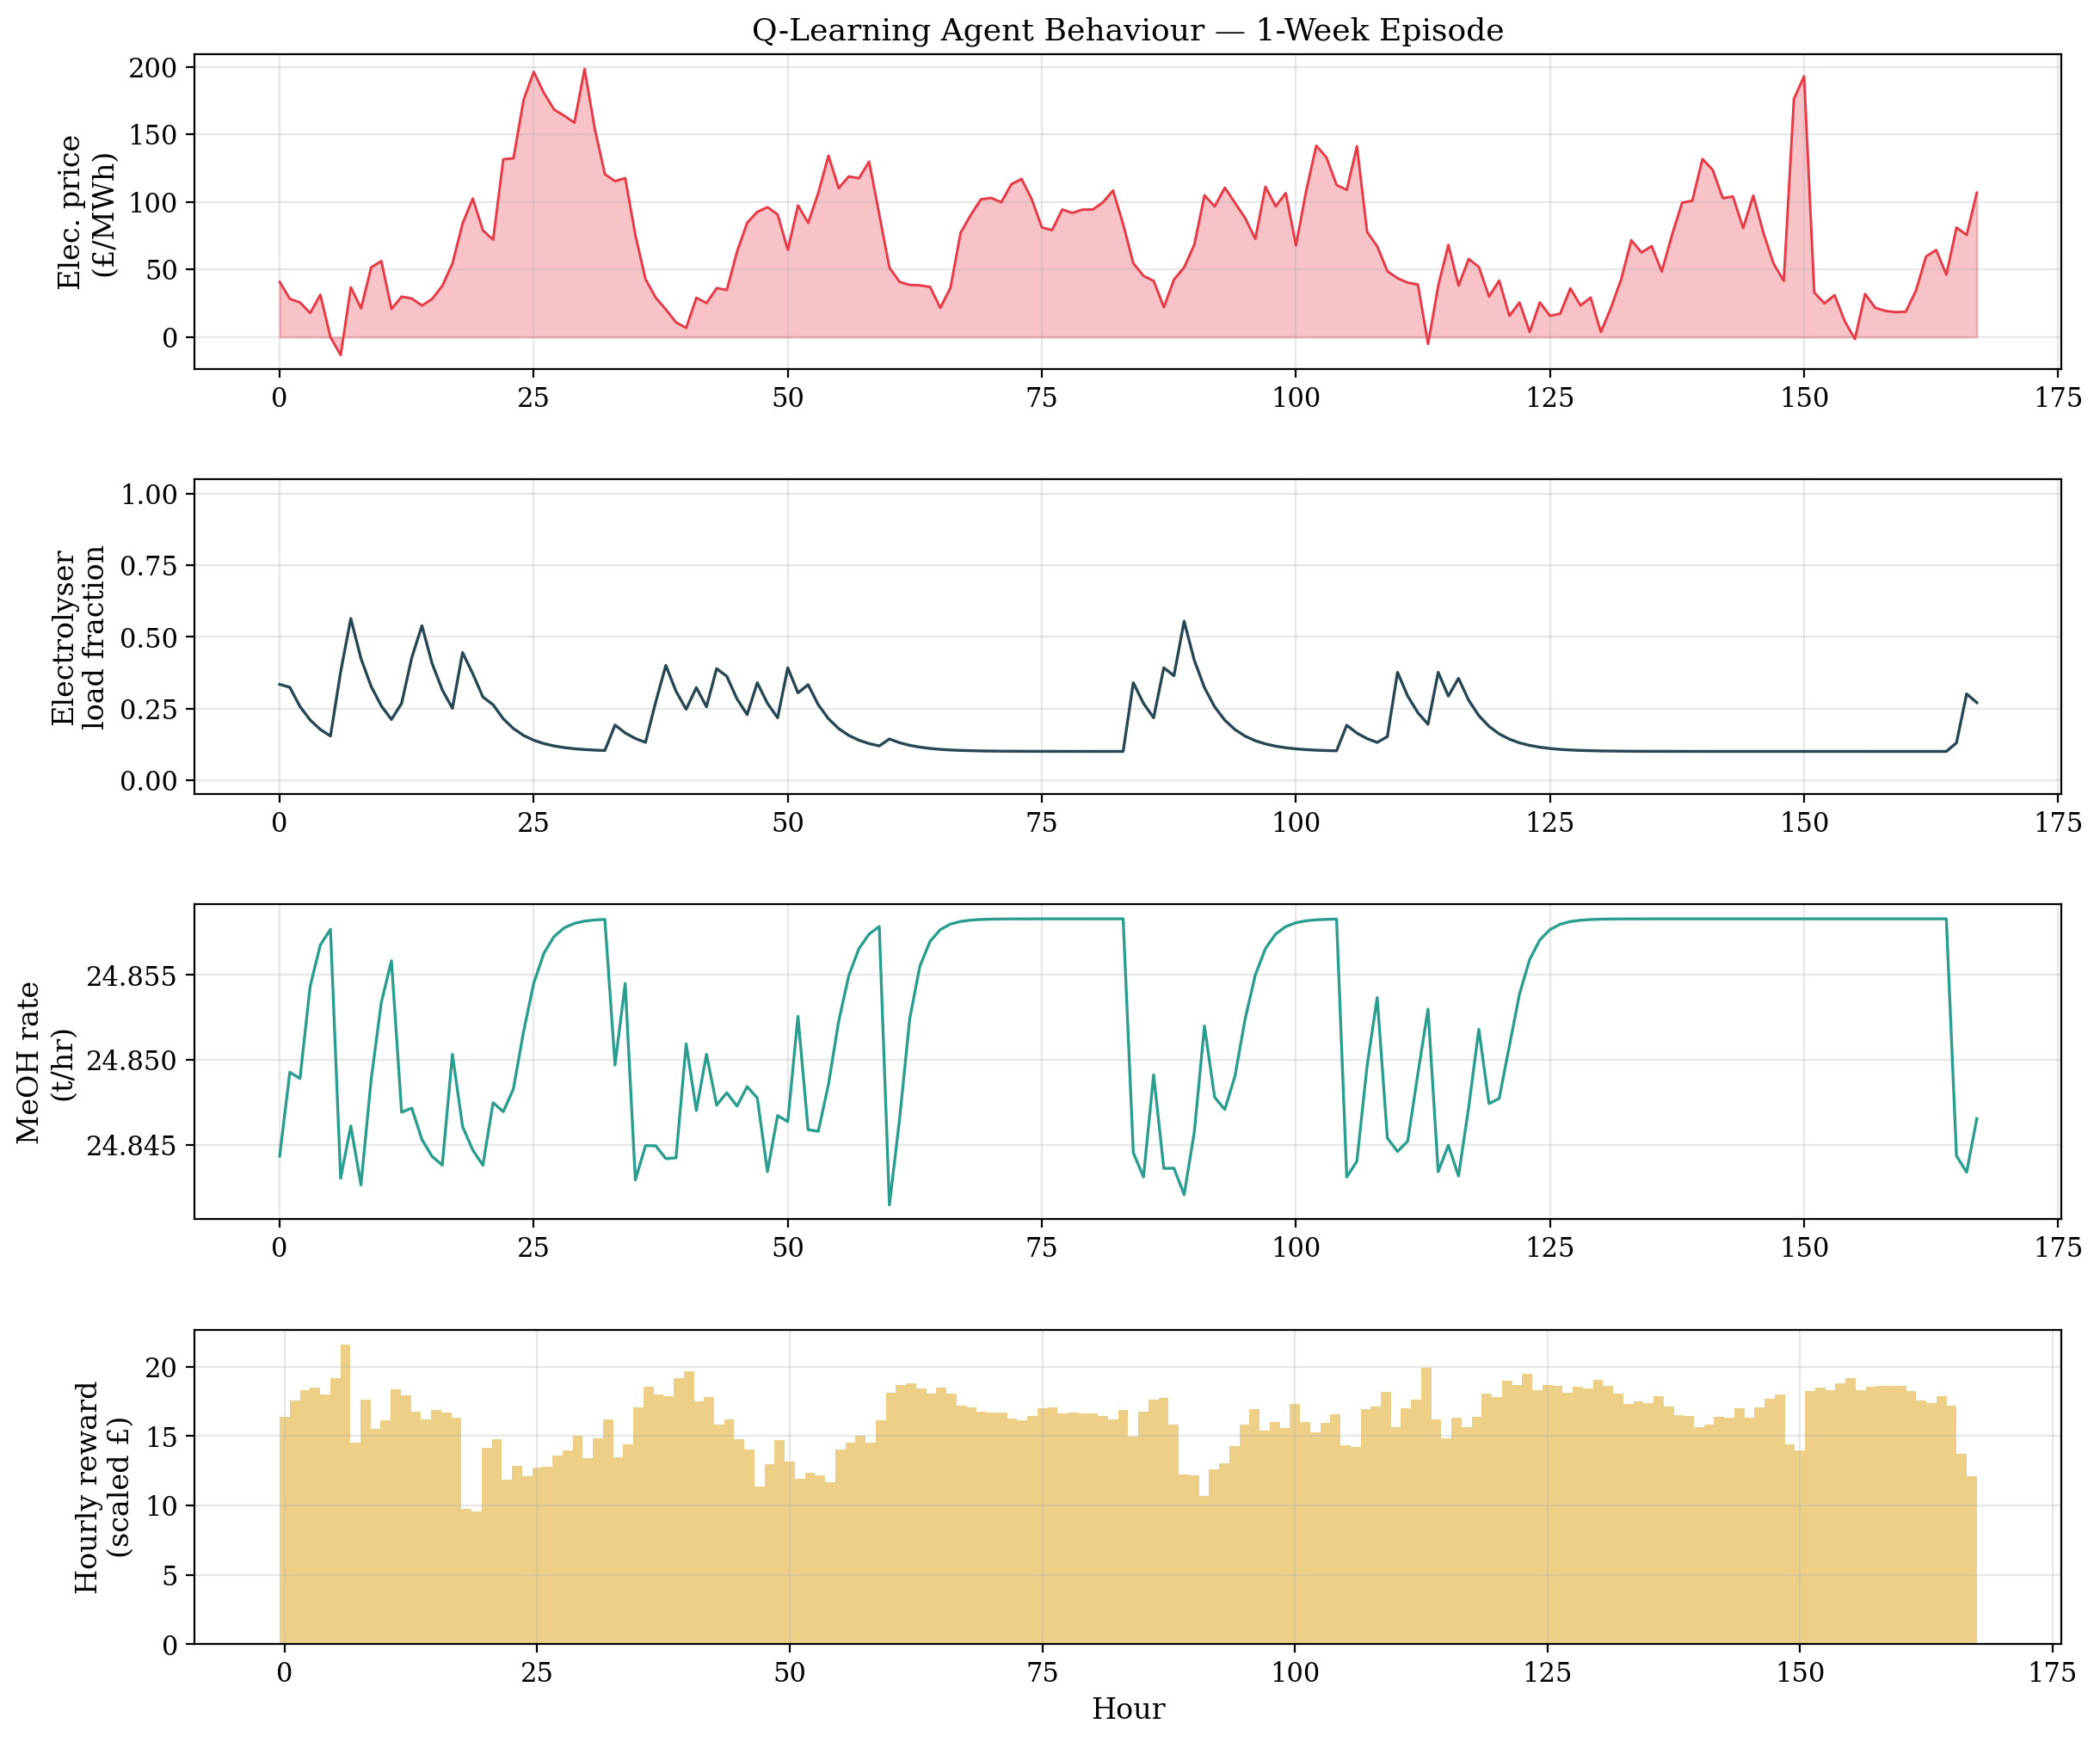
\includegraphics[width=0.72\textwidth]{figures/fig_agent_behaviour.png}
  \caption{Representative learned dispatch behaviour over a 168-hour episode.
           The qualitative control pattern is curtailment during high-price
           hours and higher operation during cheap hours.}
  \label{fig:behaviour}
\end{figure}

% ============================================================
\section{Cross-Market Transfer}

The price loader supports GB synthetic prices and Dutch ENTSO-E-style
2023--2024 price data. The transfer experiment trains SAC, PPO, and
Q-learning on GB or NL and evaluates each agent on both markets. These are
original-surrogate transfer tests, so their absolute reward values inherit
the v1 extrapolation caveat. The ranking and transfer pattern are still
useful: SAC is the strongest transferred policy, and reward changes little
when moving GB-trained SAC to NL prices.

\begin{figure}[H]
  \centering
  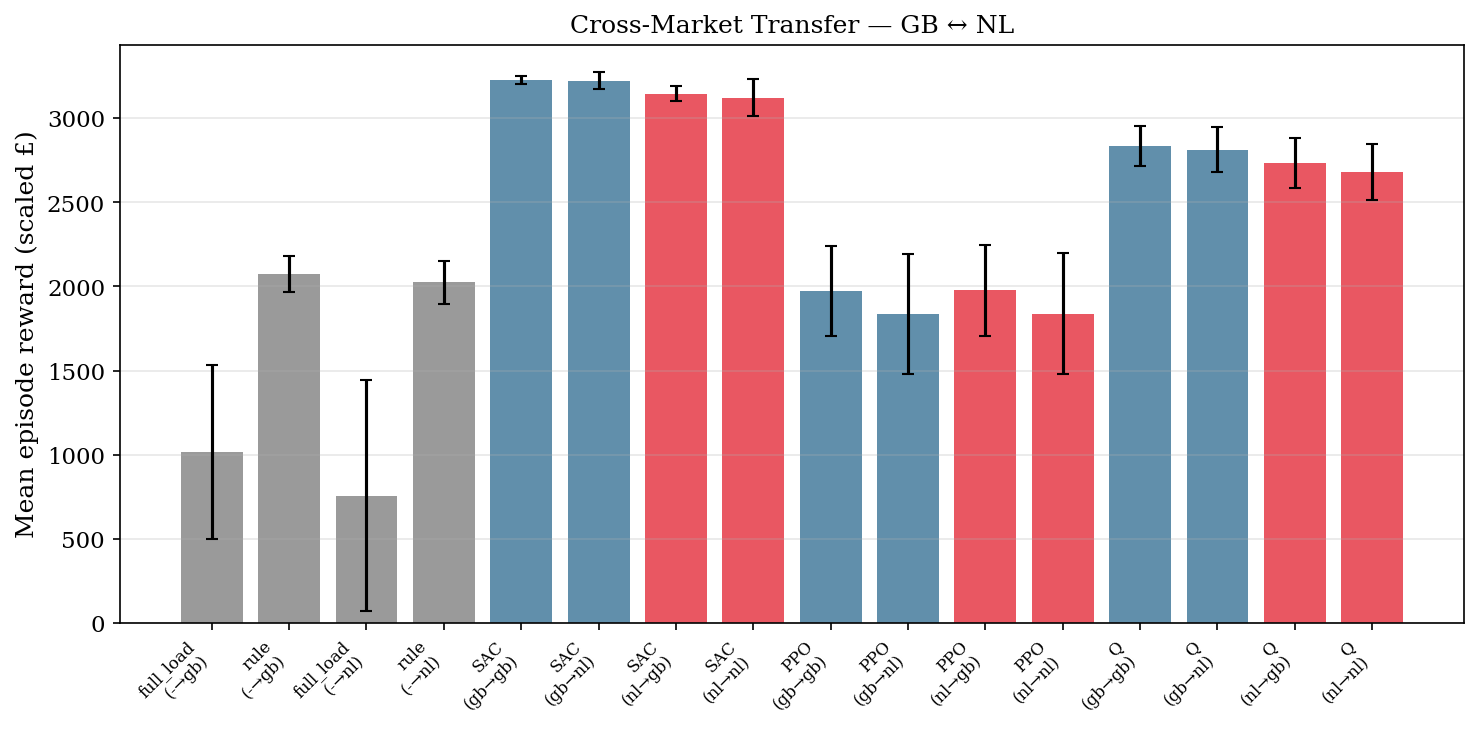
\includegraphics[width=0.85\textwidth]{figures/fig_transfer_bar.png}
  \caption{Cross-market transfer on the original surrogate setup. SAC transfers
           well across GB and NL price traces, but the absolute values should
           be read with the v1 extrapolation caveat.}
  \label{fig:transfer}
\end{figure}

\begin{table}[H]
  \centering
  \caption{Cross-market transfer matrix (mean weekly reward $\pm$ std).}
  \label{tab:transfer}
  \small
  \begin{tabular}{l rrrr}
    \toprule
    \textbf{Agent} & \textbf{GB$\to$GB} & \textbf{GB$\to$NL}
                   & \textbf{NL$\to$GB} & \textbf{NL$\to$NL} \\
    \midrule
    SAC        & $3227\pm26$  & $3222\pm50$  & $3146\pm42$  & $3123\pm112$ \\
    PPO        & $1972\pm267$ & $1838\pm355$ & $1976\pm273$ & $1839\pm358$ \\
    Q-learning & $2836\pm120$ & $2814\pm134$ & $2735\pm149$ & $2682\pm167$ \\
    \bottomrule
  \end{tabular}
\end{table}

The GB-trained SAC changes from 3227 on GB to 3222 on NL, approximately
0.1\% degradation. The NL-trained SAC also remains within 3\% when evaluated
on GB. A temporal robustness study on NL folds points in the same direction:
the GB-trained zero-shot SAC scores 3180--3287 across held-out folds, while
fold-retrained SAC ranges from 2328--3198. This supports the practical idea
that a policy trained on a broad price distribution can transfer across
nearby electricity markets, pending the surrogate validation caveat.

% ============================================================
\section{Surrogate Extrapolation Diagnosis and Correction}

\subsection{Original Problem}

The environment flags GPR extrapolation when the MeOH surrogate predictive
standard deviation exceeds twice the mean training-set standard deviation.
The original SAC triggers this warning on 96.1\% of GB evaluation steps. The
agent has converged to a low-load, high-temperature, high-pressure region
that the original 500-point LHS did not cover. Therefore, the original SAC
reward is best interpreted as an optimistic pre-correction diagnostic, not as
an Aspen-checked profit estimate.

\begin{figure}[H]
  \centering
  \begin{subfigure}[t]{0.48\textwidth}
    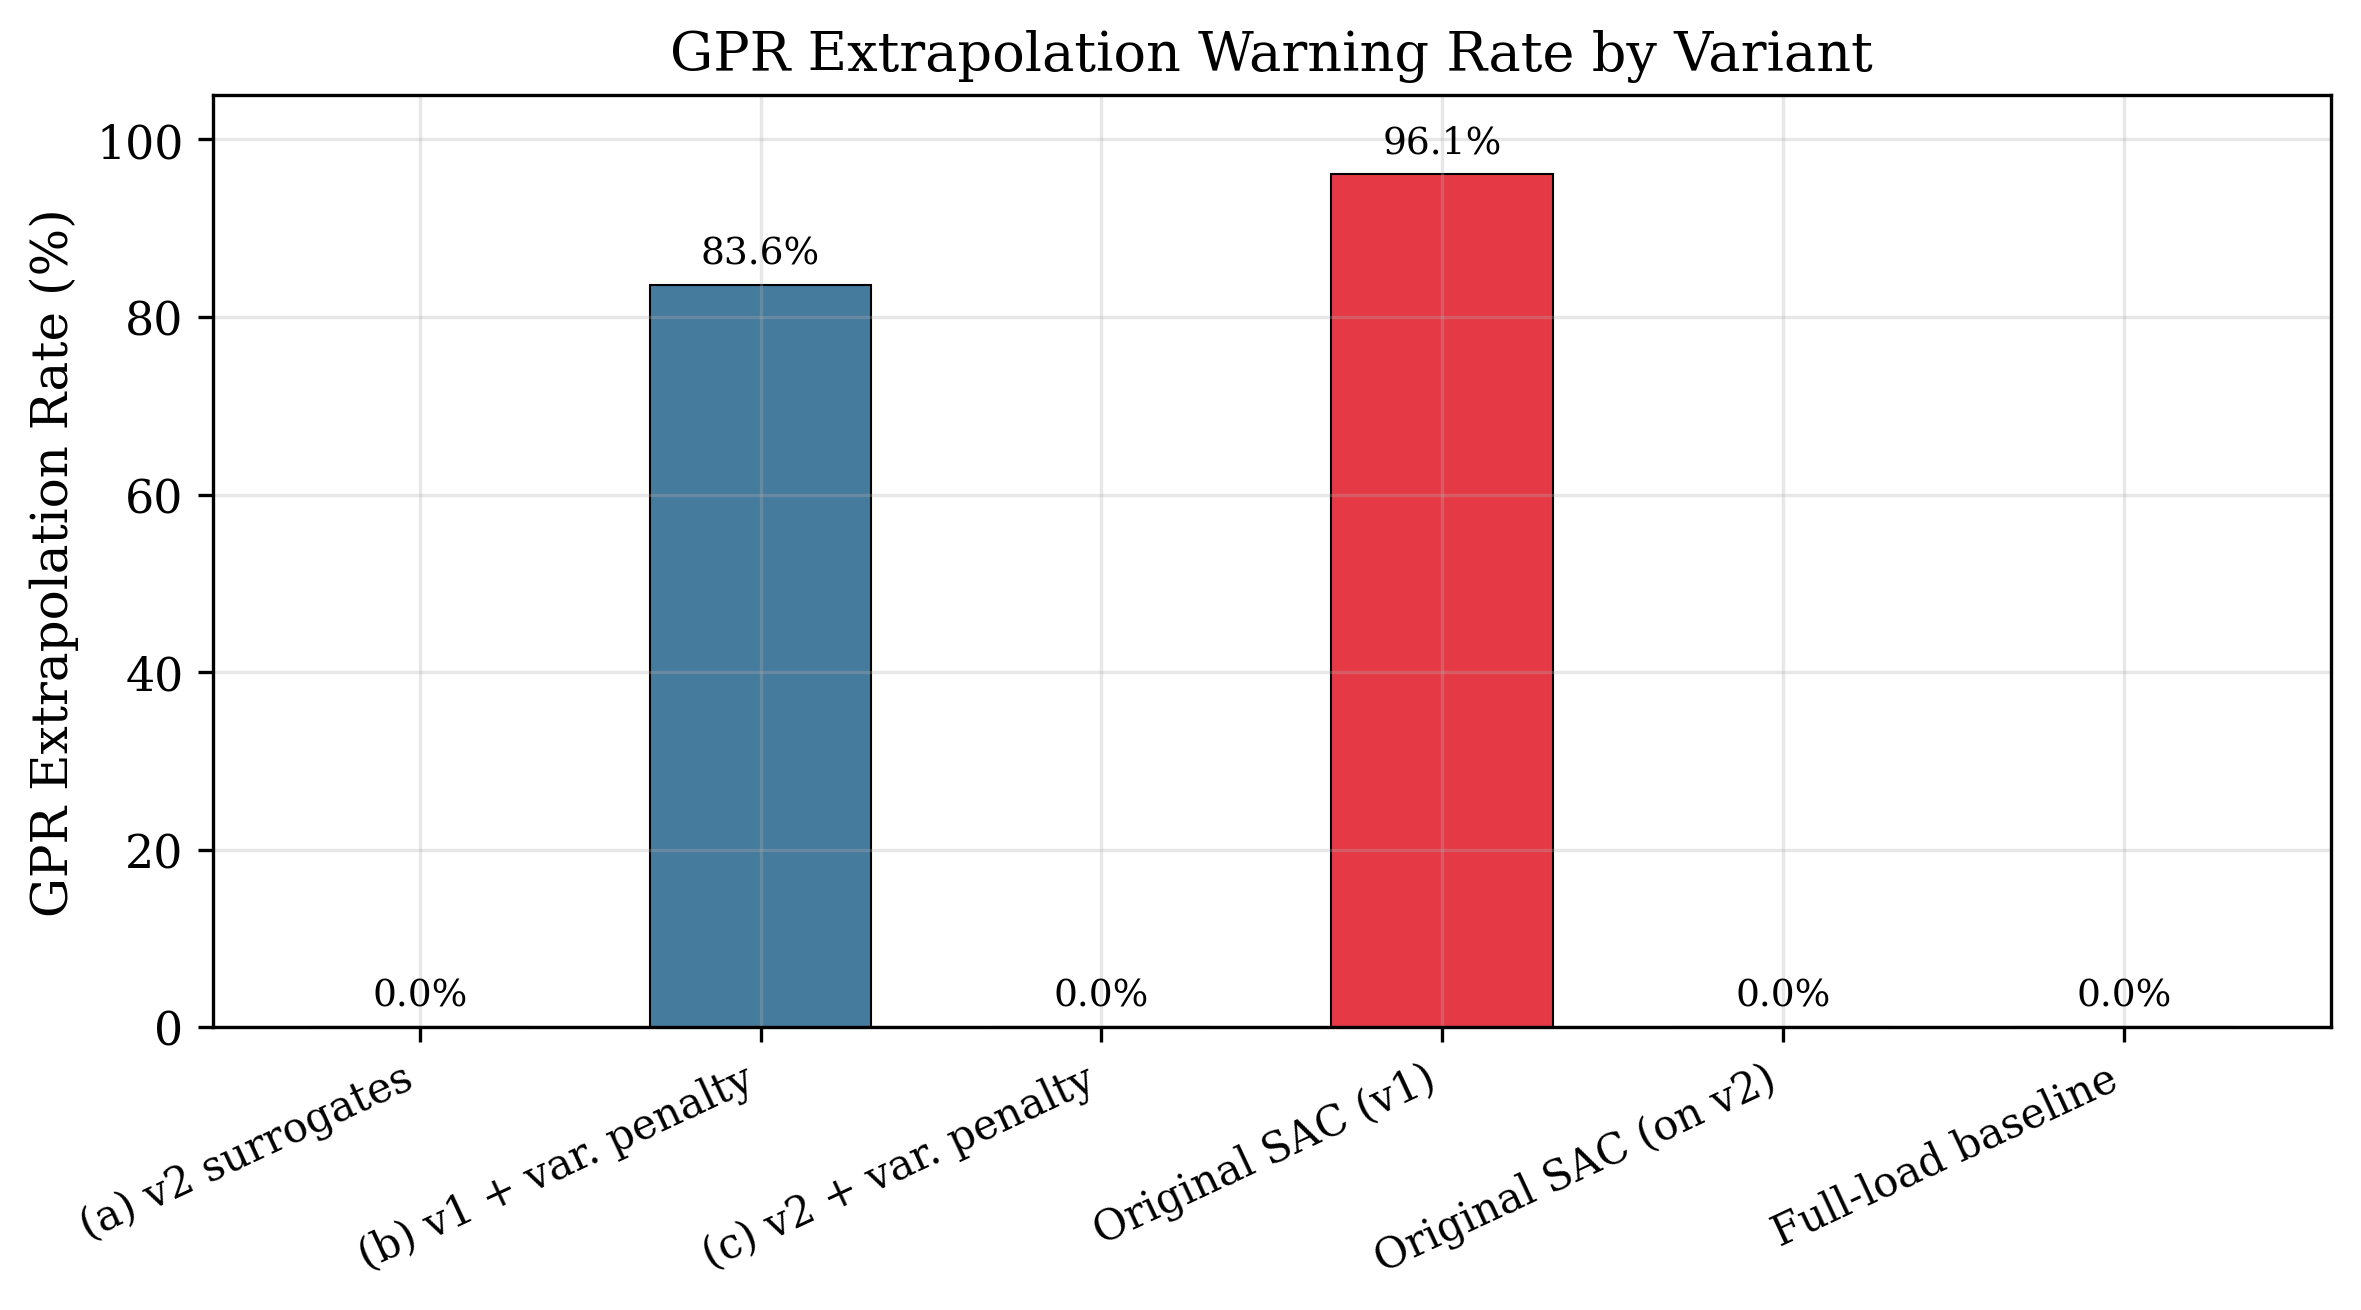
\includegraphics[width=\textwidth]{figures/fig_extrap_rate.png}
    \caption{Warning rate.}
  \end{subfigure}
  \hfill
  \begin{subfigure}[t]{0.48\textwidth}
    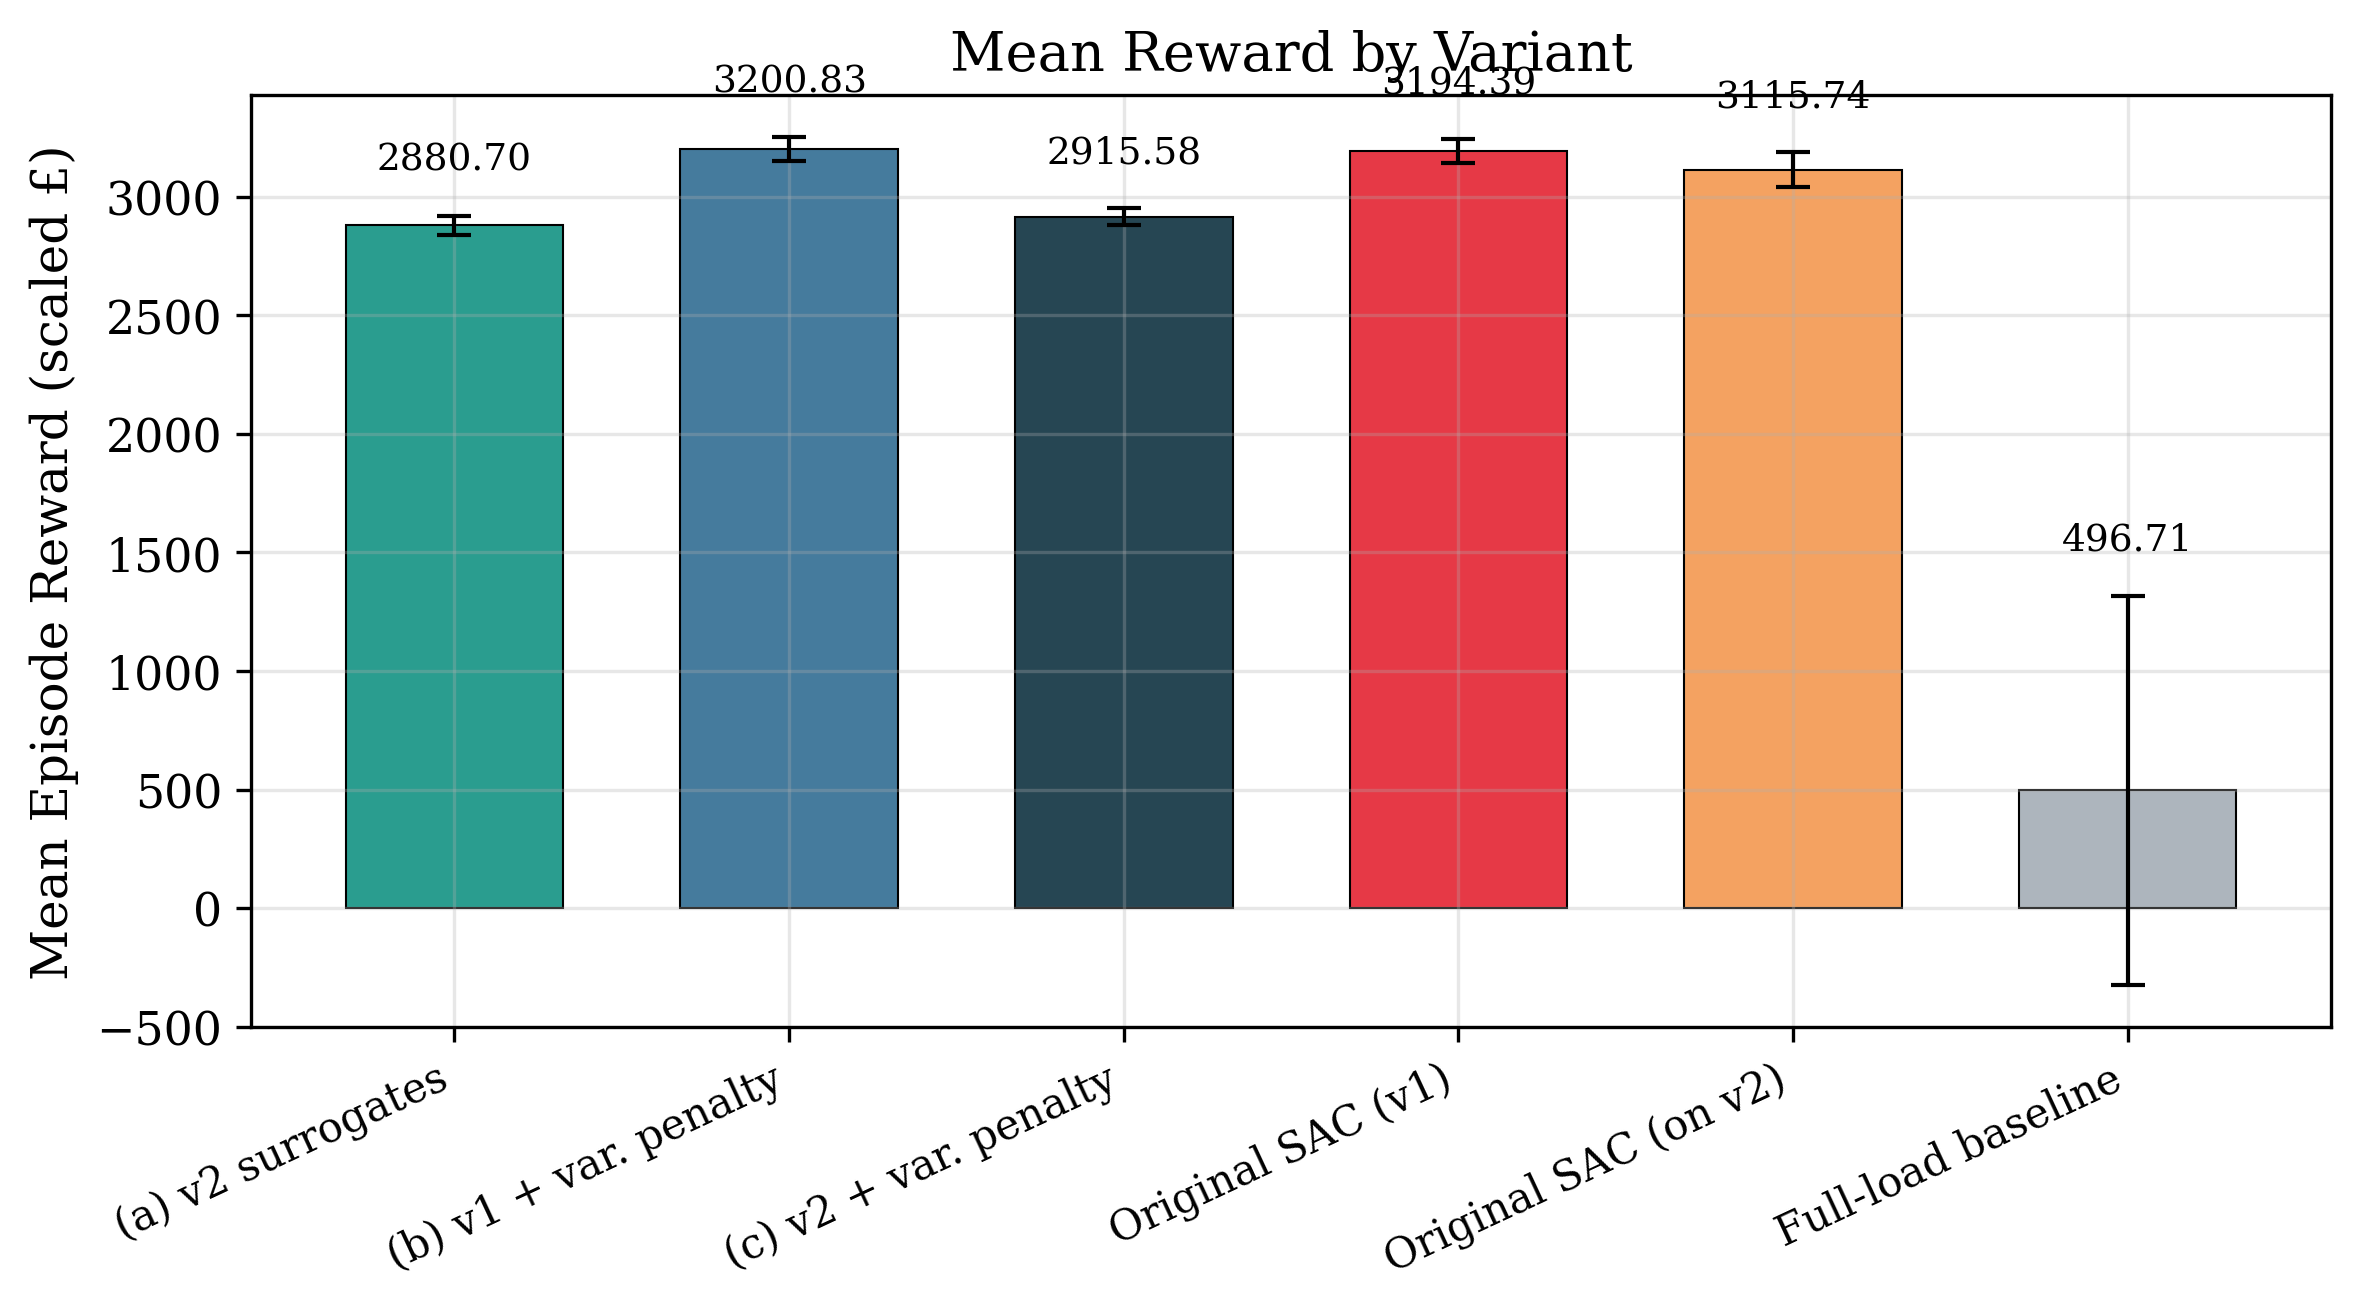
\includegraphics[width=\textwidth]{figures/fig_extrap_reward.png}
    \caption{Episode reward.}
  \end{subfigure}
  \caption{Extrapolation-fix comparison. v2 surrogate coverage removes the
           warning; the v1 variance penalty alone does not.}
  \label{fig:extrap_fix}
\end{figure}

\subsection{v2 Correction}

The v2 correction retrains surrogate models on the original 500 LHS points
plus 300 pseudo-labelled points biased toward the agent trajectory. The
labels come from the simplified process model, not Aspen. Approach~B adds a
variance penalty, but the main correction is the wider v2 surrogate coverage.

\begin{table}[H]
  \centering
  \caption{Extrapolation-fix variants. Source:
           \texttt{extrapolation\_fix\_results.csv}.}
  \label{tab:extrap}
  \small
  \begin{tabular}{l cc rrrr}
    \toprule
    \textbf{Variant} & \textbf{Surr.} & \textbf{Penalty}
      & \textbf{Reward} & \textbf{Std} & \textbf{CO\textsubscript{2} util.}
      & \textbf{Extrap.} \\
    \midrule
    Original SAC       & v1 & No  & 3194.4 & 52.1 & 0.935 & 96.1\% \\
    Original on v2     & v2 & No  & 3115.7 & 74.2 & 0.916 & 0.0\% \\
    Fix~(a)            & v2 & No  & 2880.7 & 39.8 & 0.836 & 0.0\% \\
    Fix~(b)            & v1 & Yes & 3200.8 & 50.6 & 0.935 & 83.6\% \\
    Fix~(c)            & v2 & Yes & 2915.6 & 35.8 & 0.848 & 0.0\% \\
    Full-load baseline & v1 & No  & 496.7  & 821.2 & 0.938 & 0.0\% \\
    \bottomrule
  \end{tabular}
\end{table}

\begin{figure}[H]
  \centering
  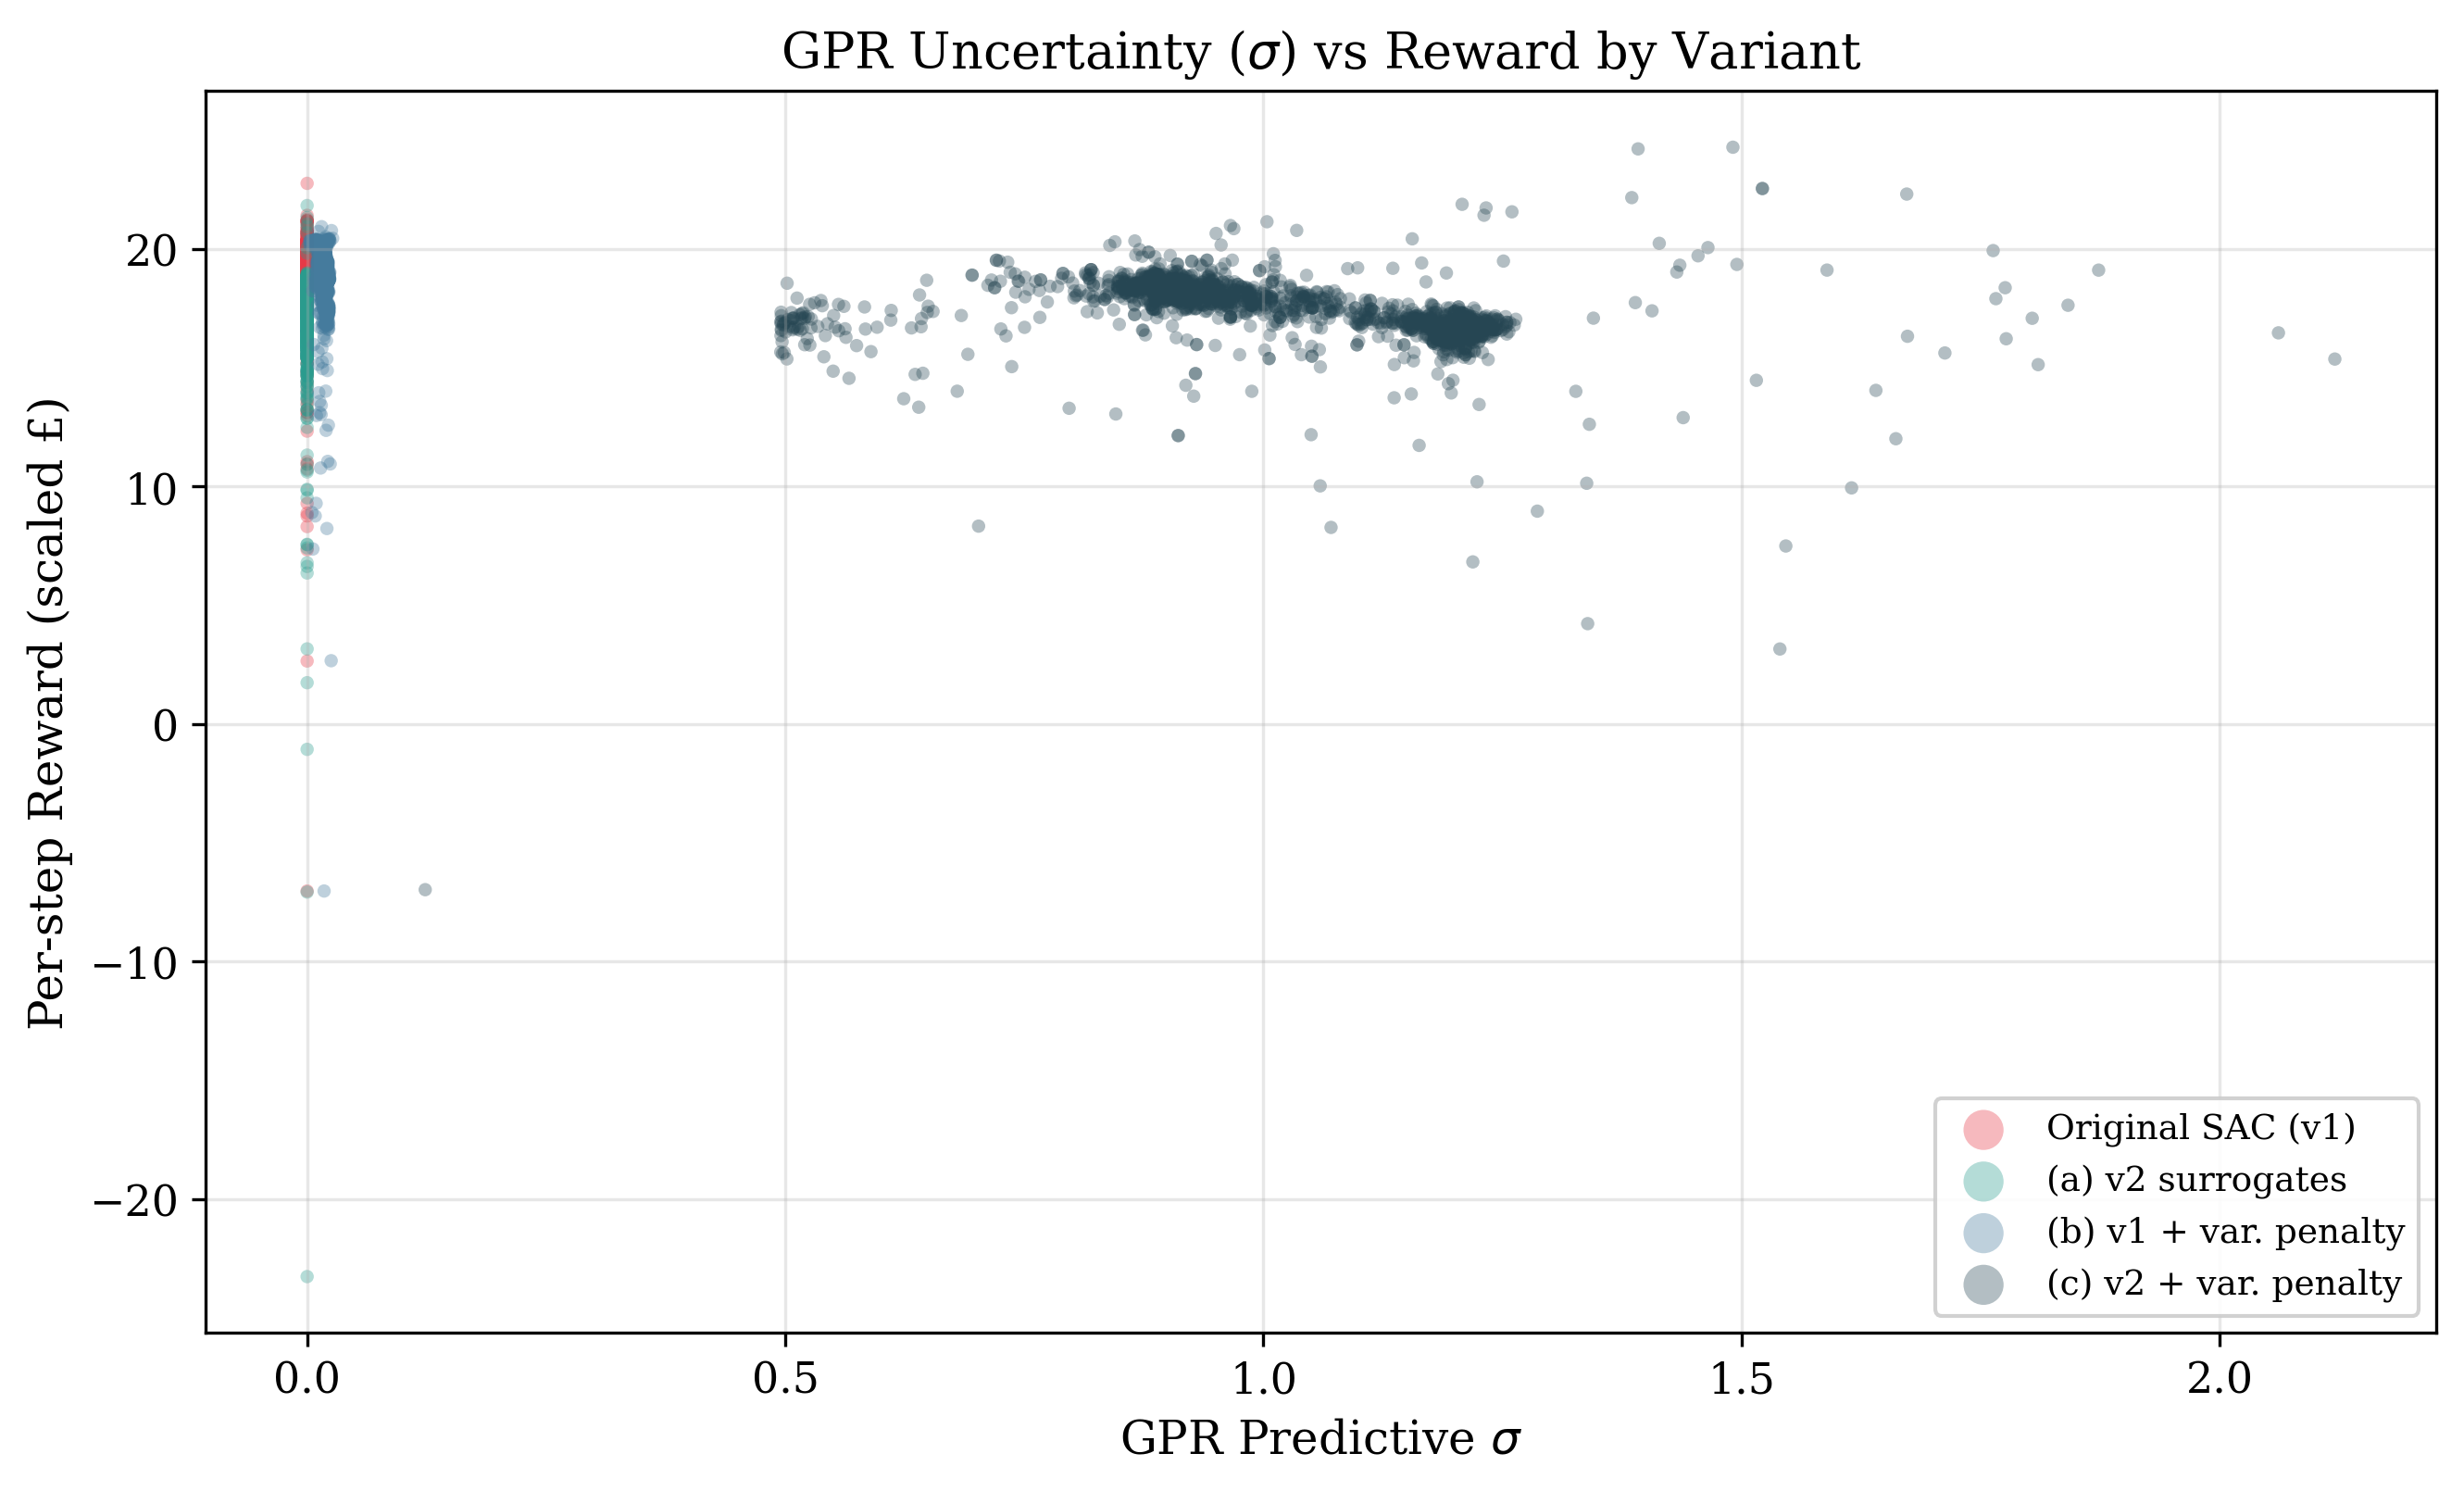
\includegraphics[width=0.78\textwidth]{figures/fig_sigma_vs_reward.png}
  \caption{GPR predictive $\sigma$ versus per-step reward. The original SAC
           occupies high-$\sigma$ regions; v2 policies move into the corrected
           surrogate coverage.}
  \label{fig:sigma}
\end{figure}

\begin{figure}[H]
  \centering
  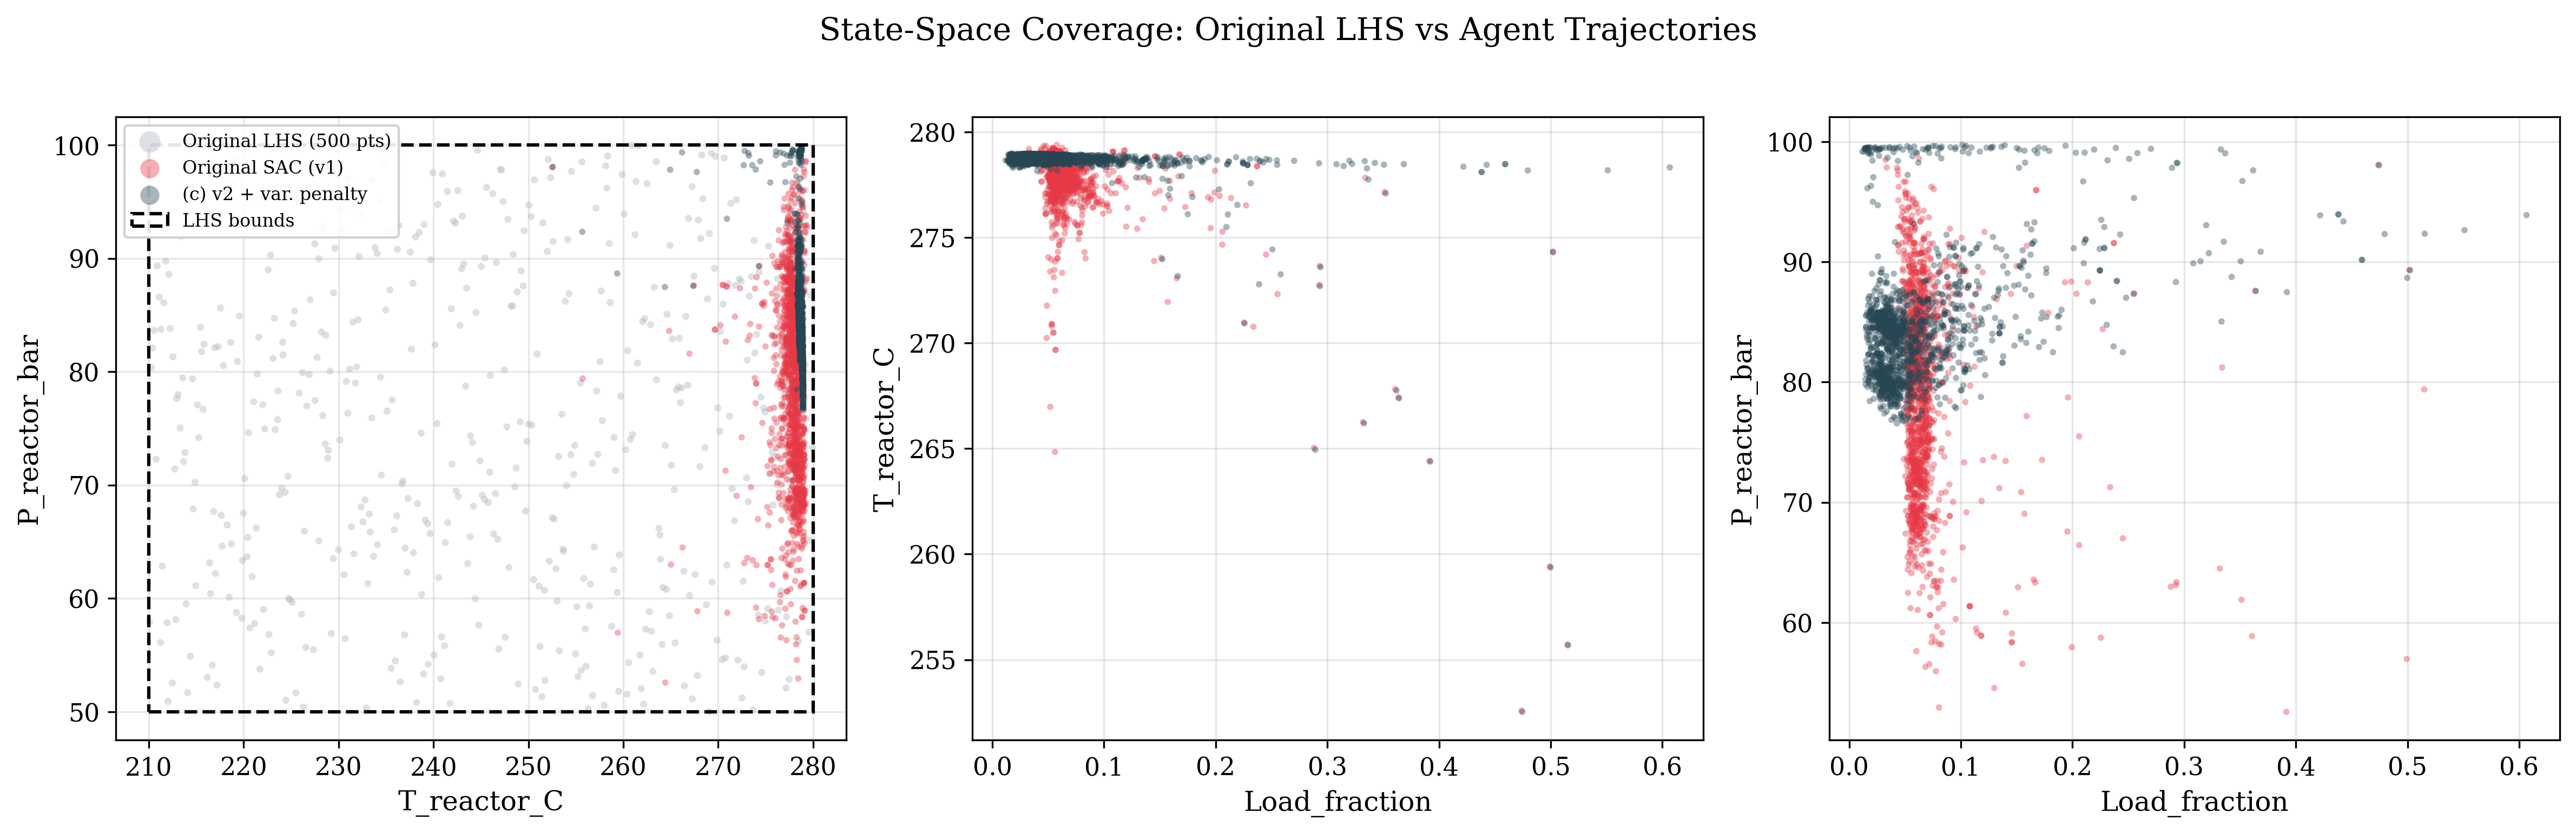
\includegraphics[width=0.9\textwidth]{figures/fig_state_space.png}
  \caption{State-space coverage in $T$--$P$, load--$T$, and load--$P$
           projections. The discovered SAC operating region lies away from the
           original LHS; v2 is a pseudo-labelled attempt to cover that region.}
  \label{fig:state_space}
\end{figure}

The honest interpretation is that v2 gives an internally consistent corrected
evaluation. It removes the warning and retains large RL value, but it cannot
by itself establish physical accuracy in the low-load region because the new
labels were not produced by Aspen.

\subsection[v3 Extended FH2 Domain]{v3 Extended $F_{\mathrm{H}_2}$ Domain}

GNN diagnostics exposed a second surrogate issue: the original 5-D LCOM GPR
was fitted on $F_{\mathrm{H}_2} \in [2515, 3147]$~kmol/hr, while the dynamic
pipeline can map low PEM capacity factors to much lower
$F_{\mathrm{H}_2}$ values. The v3 saved surrogates extend the fitted
LCOM/utility domain using 500 additional pseudo-labelled LHS points with
$F_{\mathrm{H}_2} \in [800, 3200]$~kmol/hr, combined with the original 500
points.

\begin{table}[H]
  \centering
  \caption{v3 held-out fit metrics from
           \texttt{outputs/surrogate\_v3/summary.json}. These are surrogate
           fit metrics against pseudo-labels, not Aspen validation metrics.}
  \label{tab:v3}
  \small
  \begin{tabular}{l cc}
    \toprule
    \textbf{GPR target} & \textbf{Test $R^2$} & \textbf{Test RMSE} \\
    \midrule
    LCOM                & 0.99981 & 0.98 \pounds/t \\
    Utility             & 0.99936 & $1.1 \times 10^{-3}$ \\
    \bottomrule
  \end{tabular}
\end{table}

When the v2-trained Fix~(c) policy is scored on v3 without retraining, mean
reward collapses to $-161.6 \pm 6.4$ with 0\% extrapolation. This is not a
failure of SAC as an algorithm; it shows that the low-load
$F_{\mathrm{H}_2}$ domain is economically important and that the previous v2
policy was not trained on the latest intended v3 surface. The v3 result requires
fresh SAC retraining and Aspen low-load spot checks before updated economic
claims can be made.

% ============================================================
\section{GNN Flowsheet Surrogate Extension}

\subsection{Graph-Level KPI Failure}

A topology-aware GINE model was first tested as a direct graph-to-KPI
surrogate for [TAC, carbon efficiency, LCOM]. The best graph-level
configuration fits TAC and carbon efficiency reasonably well but fails on
LCOM. This is an informative ablation: LCOM is a low-dimensional
position-specific GPR distillation, and graph-level mean/add pooling discards
the positional information required to reconstruct it.

\begin{figure}[H]
  \centering
  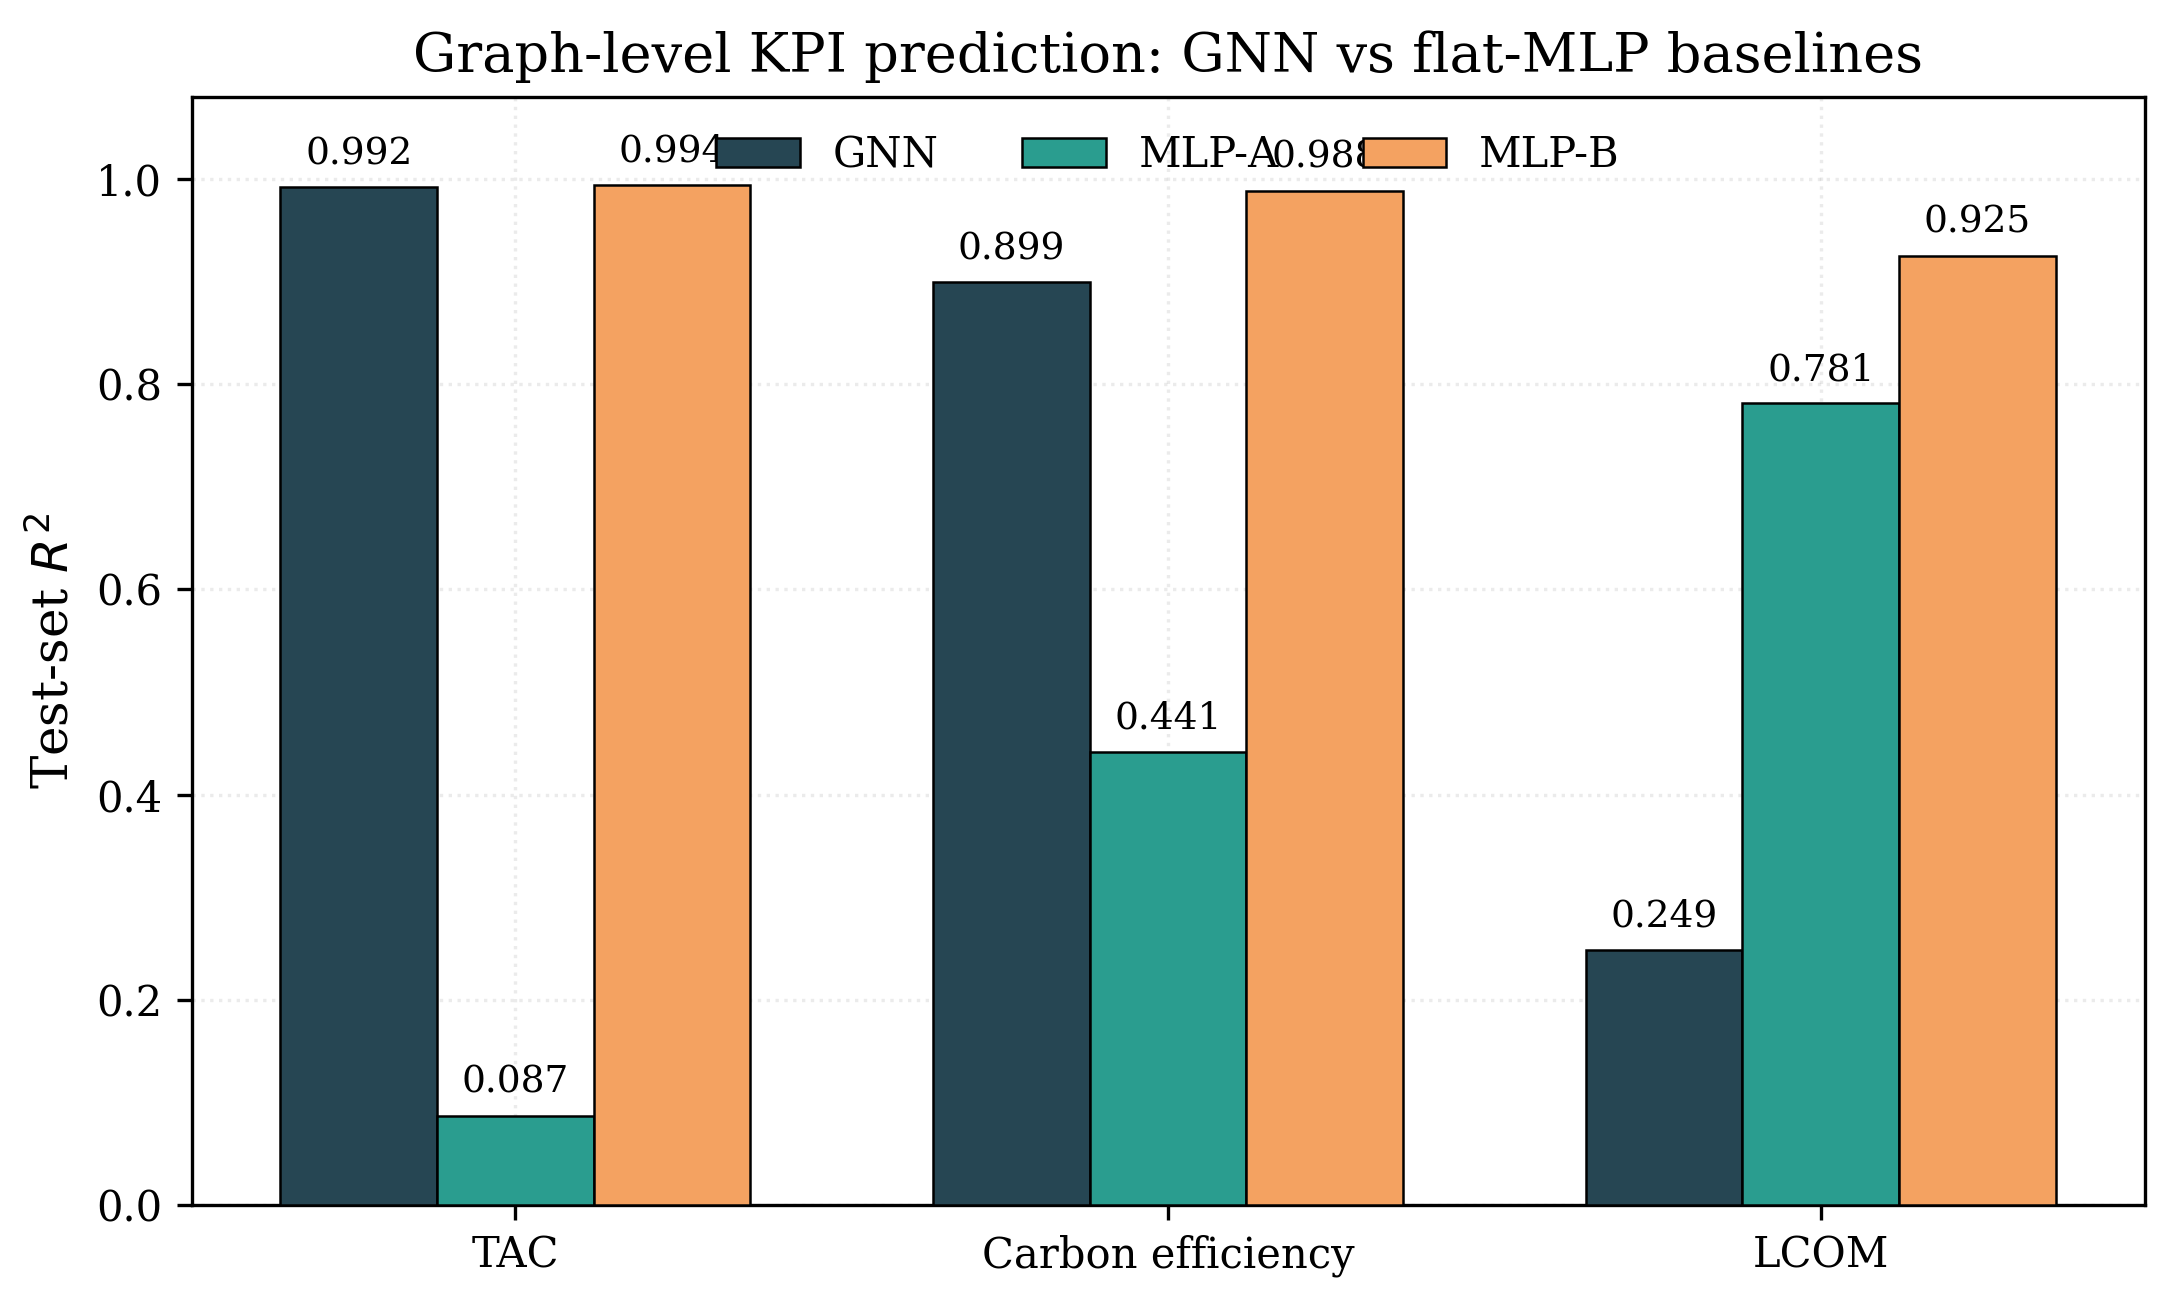
\includegraphics[width=0.82\textwidth]{figures/fig_gnn_comparison.png}
  \caption{Graph-level KPI prediction. The GNN under-fits LCOM; flat MLP
           baselines reveal that this is a task-formulation mismatch, not just
           a lack of learnable signal.}
  \label{fig:gnn_compare}
\end{figure}

\begin{table}[H]
  \centering
  \caption{Graph-level KPI regression and flat baselines. The edge-augmented
           MLP result is not treated as a production model because edge mass
           flows leak production information into the input.}
  \label{tab:gnn_compare}
  \small
  \begin{tabular}{l ccc}
    \toprule
    \textbf{Model} & $\mathbf{R^2_{\mathrm{TAC}}}$ &
    $\mathbf{R^2_{\mathrm{carbon}}}$ & $\mathbf{R^2_{\mathrm{LCOM}}}$ \\
    \midrule
    GNN (best graph-level config) & 0.992 & 0.899 & 0.249 \\
    MLP-A (design only)           & 0.087 & 0.441 & 0.781 \\
    MLP-B (design + edge-flat)    & 0.994 & 0.988 & 0.925 \\
    Cap-factor fix GNN            & 0.991 & 0.894 & 0.375 \\
    \bottomrule
  \end{tabular}
\end{table}

\subsection{Edge-State Reframe}

The successful reframe is per-edge state prediction. The model predicts eight
physical quantities for each of 13 edges:
\[
\left[\dot{m}, T, P, x_{\mathrm{CO_2}}, x_{\mathrm{H_2}},
x_{\mathrm{MeOH}}, x_{\mathrm{H_2O}}, x_{\mathrm{inert}}\right].
\]
The two structural flags (\texttt{is\_recycle}, \texttt{is\_energy}) remain
as edge inputs, while physical edge quantities are moved to the target to
avoid leakage. This aligns the learning task with graph message passing.

\begin{figure}[H]
  \centering
  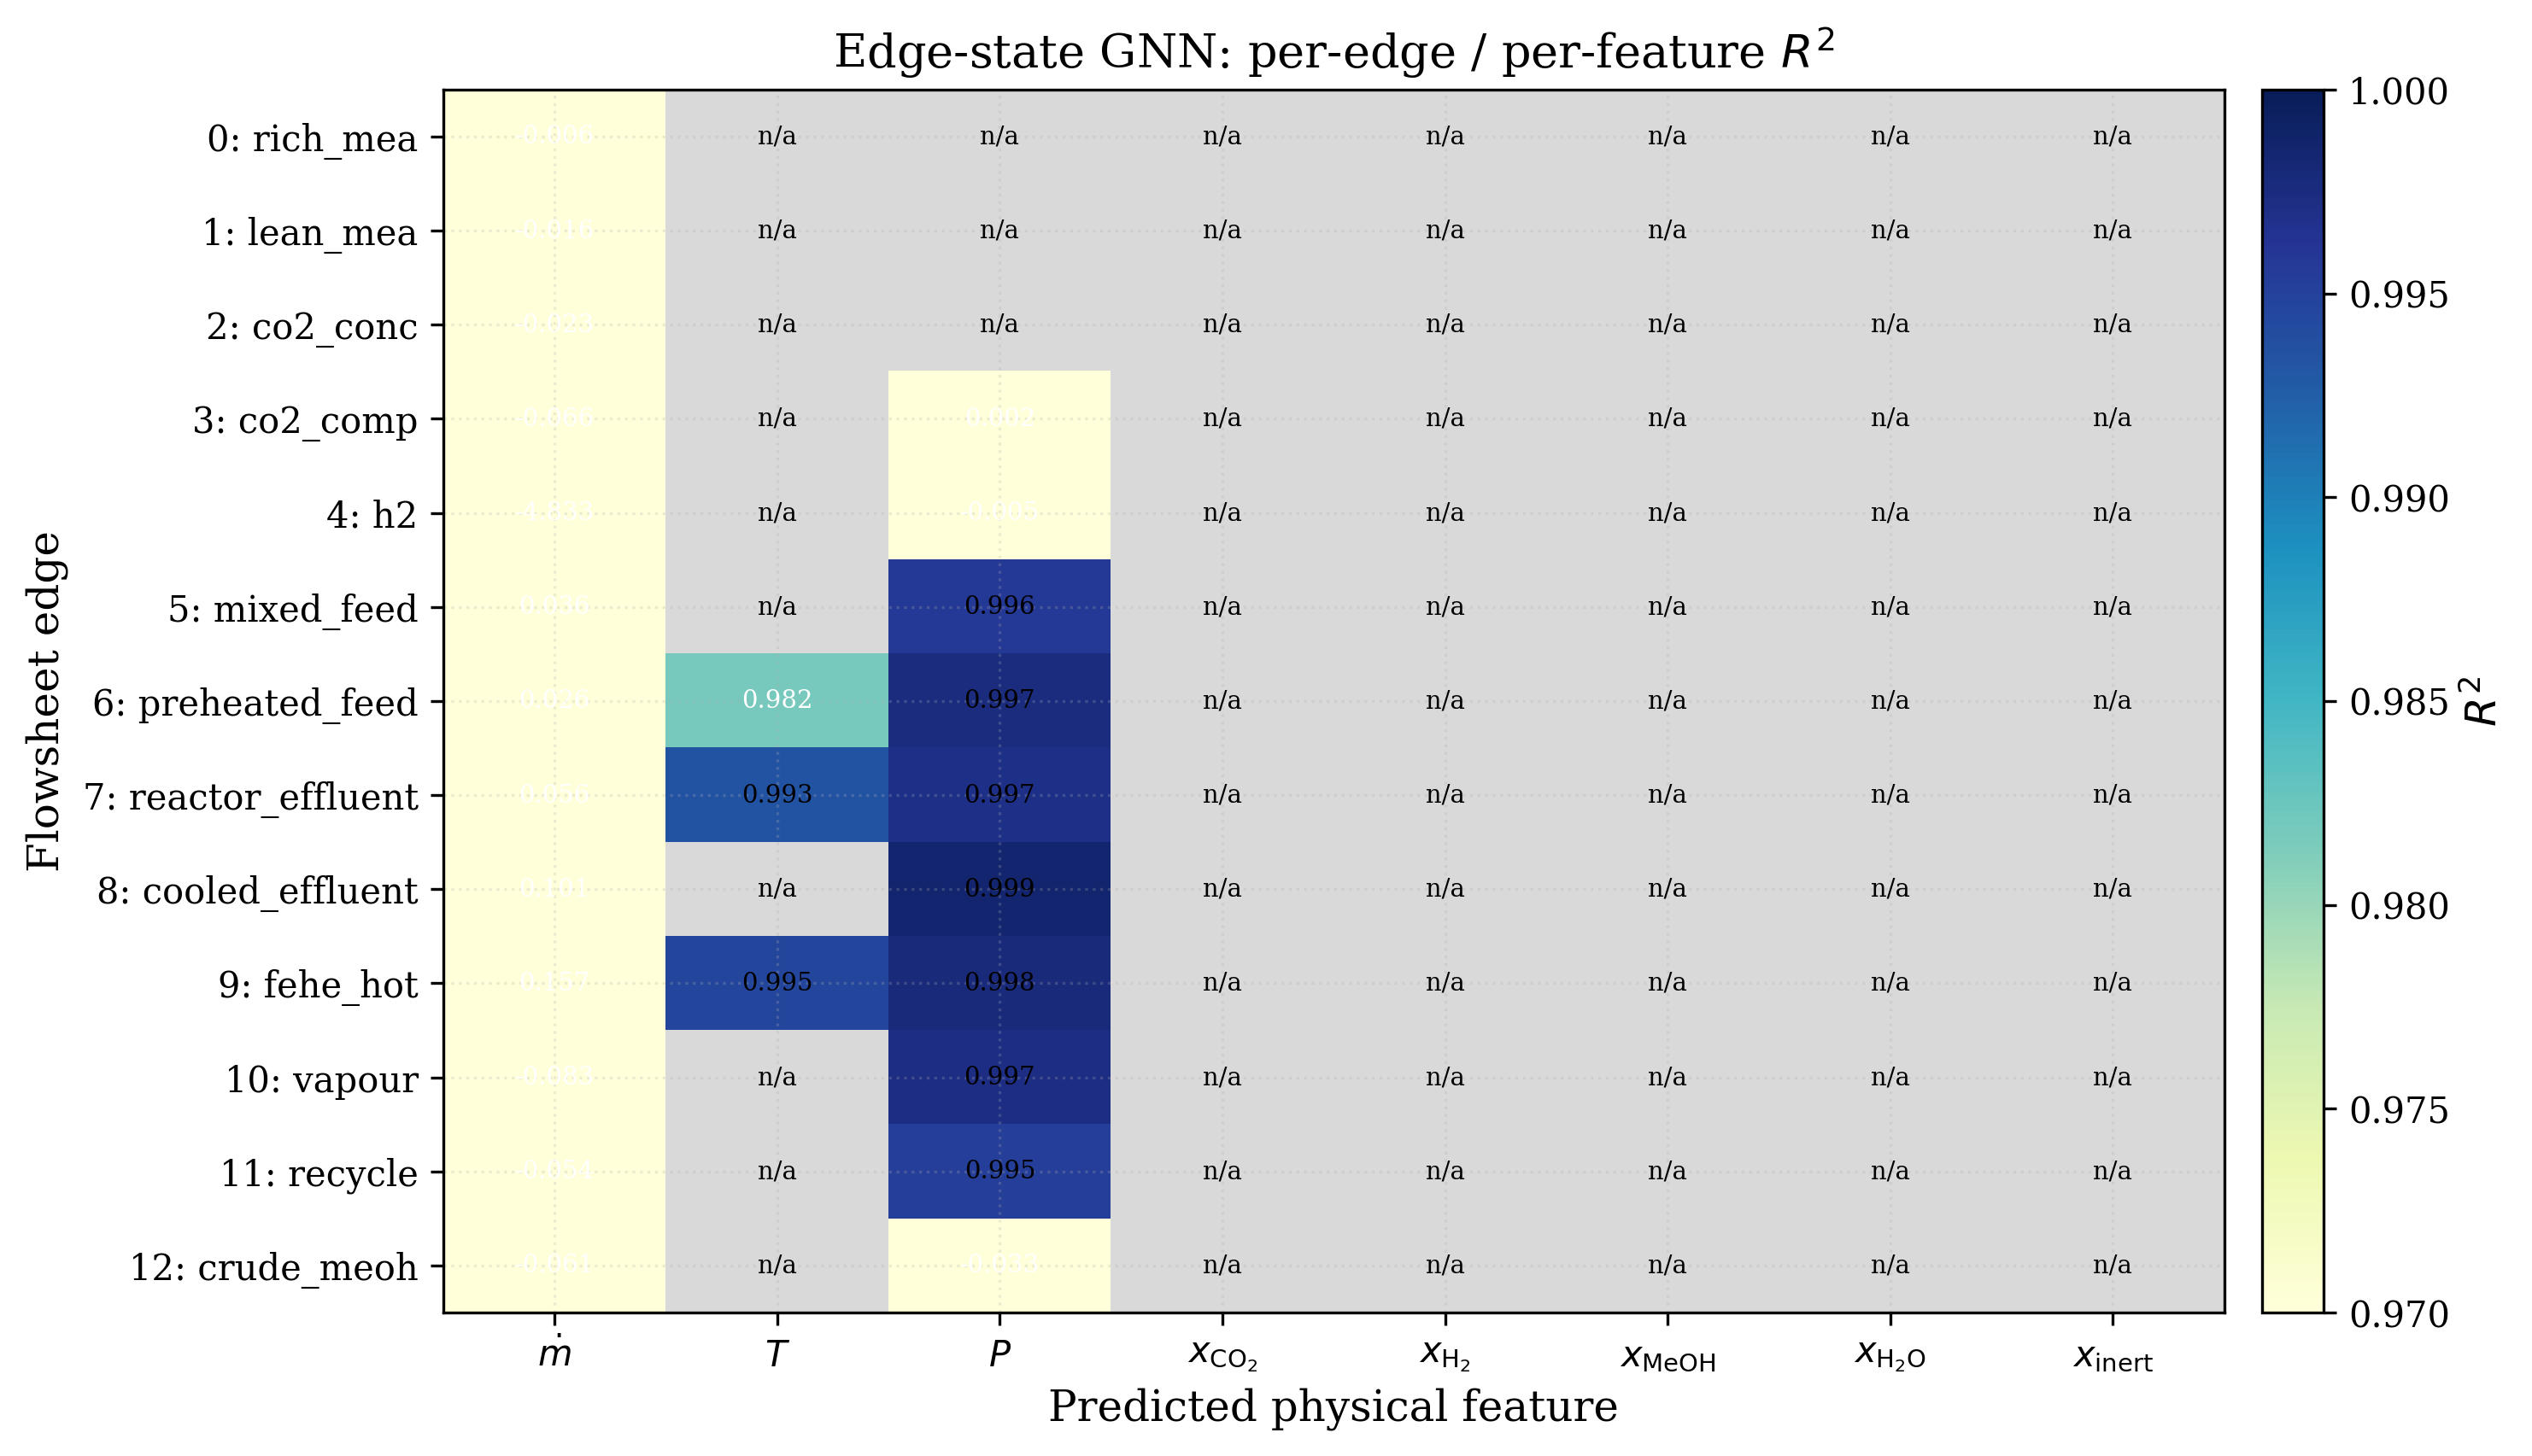
\includegraphics[width=0.86\textwidth]{figures/fig_edge_heatmap.png}
  \caption{Per-edge/per-feature $R^2$ map for the edge-state GNN. Most
           informative physical channels are fitted at very high accuracy.}
  \label{fig:edge_heatmap}
\end{figure}

\begin{figure}[H]
  \centering
  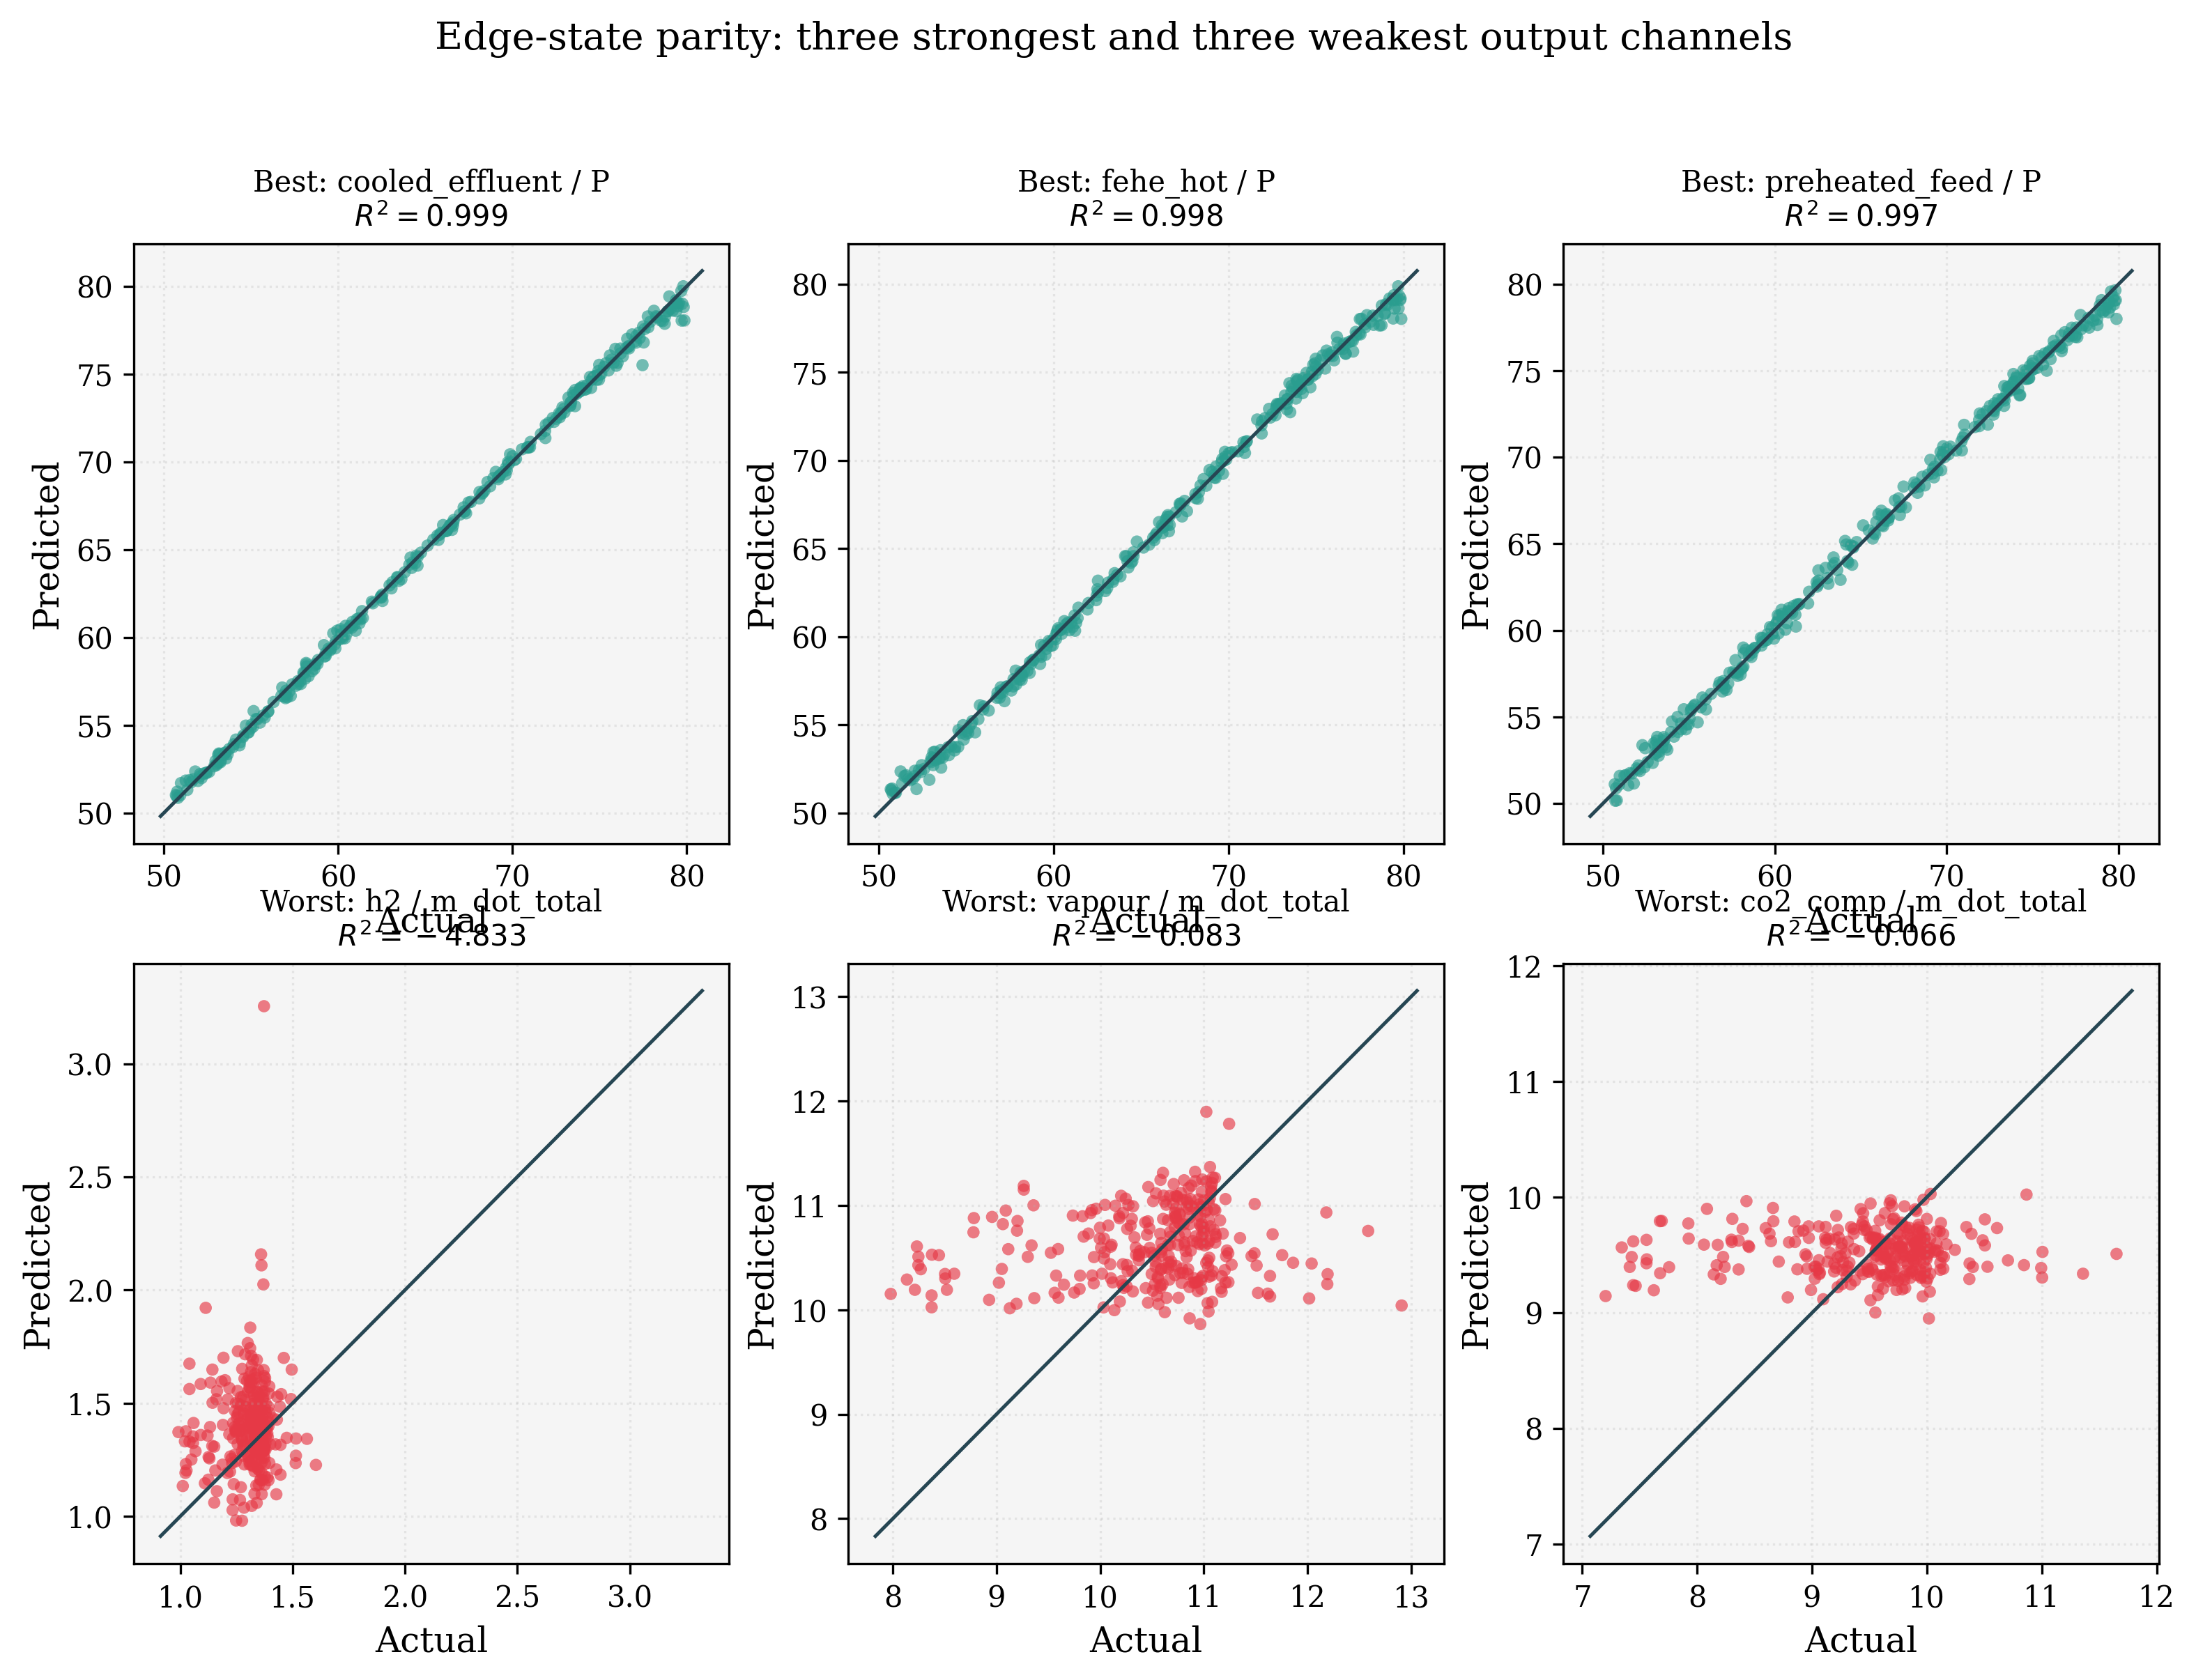
\includegraphics[width=0.9\textwidth]{figures/fig_edge_parity.png}
  \caption{Parity plots for selected edge-state channels. The edge-state task
           avoids the direct graph-level LCOM collapse.}
  \label{fig:edge_parity}
\end{figure}

The result is strong for plant-state prediction: mean per-edge $R^2$ is
0.997, worst feature $R^2$ is 0.991 for total mass flow, and temperatures
and compositions are near 0.9999. A derived methanol-rate proxy from the
distillate edge remains weak ($R^2 \approx -0.06$), so the defensible
architecture is not ``GNN directly predicts all economics''. It is:
edge-state GNN for structured plant state, scalar GPR heads for LCOM/utility,
and explicit TAC formulas where available.

% ============================================================
\section{Additional Negative Experiments}

These experiments are kept because they narrow the design space, but they do
not drive the main claim.

\subsection{PPO Fix Sweep}

The original PPO transfer results suggested a constant-policy collapse.
Four standard interventions were tested for 500k steps: larger rollout
horizon, smaller learning rate, more epochs, and VecNormalize, individually
and combined. Only the normalised variants develop nonzero load variance; all
PPO variants keep reactor temperature and pressure variance at zero.

\begin{table}[H]
  \centering
  \caption{PPO fix sweep from \texttt{outputs/ppo\_fix\_results.csv}.
           VecNormalize rows use a different reward scale from plain PPO rows.}
  \label{tab:ppo-fix}
  \small
  \resizebox{\textwidth}{!}{%
  \begin{tabular}{l l rr rrr}
    \toprule
    \textbf{Experiment} & \textbf{Algo} & \textbf{Reward} & \textbf{Std}
      & \textbf{var(load)} & \textbf{var($T$)} & \textbf{var($P$)} \\
    \midrule
    \texttt{sac\_original}      & SAC & 1139.9 & 481.0 & $1.1 \times 10^{-3}$ & 430.9 & 249.7 \\
    \texttt{ppo\_vecnormalize}  & PPO & 961.7  & 469.5 & 0.023 & 0.0 & 0.0 \\
    \texttt{ppo\_fixed\_combo}  & PPO & 934.2  & 457.1 & 0.013 & 0.0 & 0.0 \\
    \texttt{ppo\_original}      & PPO & 413.4  & 484.9 & 0 & 0 & 0 \\
    \texttt{ppo\_nsteps\_4096}  & PPO & 413.4  & 484.9 & 0 & 0 & 0 \\
    \texttt{ppo\_lr\_1e4}       & PPO & 413.4  & 484.9 & 0 & 0 & 0 \\
    \texttt{ppo\_epochs\_20}    & PPO & 413.4  & 484.9 & 0 & 0 & 0 \\
    \bottomrule
  \end{tabular}}
\end{table}

\subsection{GNN Confidence Penalty}

An edge-state GNN uncertainty penalty was added to the SAC reward on v2
surrogates. It underperforms Fix~(c): mean reward falls from 2915.6 to 719.9
and variance rises sharply. The likely reason is that the v2 GPR coverage
problem is already removed, so the GNN penalty becomes a broadly applied
negative shaping term rather than a targeted novelty penalty.

\begin{table}[H]
  \centering
  \caption{GNN-confidence penalty versus Fix~(c).}
  \label{tab:gnn-penalty}
  \small
  \begin{tabular}{l rrrrr}
    \toprule
    \textbf{Variant} & \textbf{Reward} & \textbf{Std}
      & \textbf{CO\textsubscript{2} util.} & \textbf{Extrap.}
      & $\bar{\sigma}_{\mathrm{GNN}}$ \\
    \midrule
    Fix~(c) v2 + variance penalty & 2915.6 & 35.8  & 0.848 & 0.0\%  & --- \\
    Edge-state GNN penalty        & 719.9  & 590.1 & 0.808 & 0.15\% & 0.183 \\
    \bottomrule
  \end{tabular}
\end{table}

\subsection{Pareto Degeneracy}

The profit/CO\textsubscript{2}-utilisation Pareto sweep is degenerate:
CO\textsubscript{2} utilisation stays near 93.5\% across the sweep. The
profit/electricity reframe is also mostly degenerate because electricity
cost is already inside the profit term. Eight of nine electricity-weighted
SAC runs collapse to approximately 23,615~MWh/episode; only one run jumps to
a full-load-like 45,567~MWh/episode.

\begin{figure}[H]
  \centering
  \begin{subfigure}[t]{0.48\textwidth}
    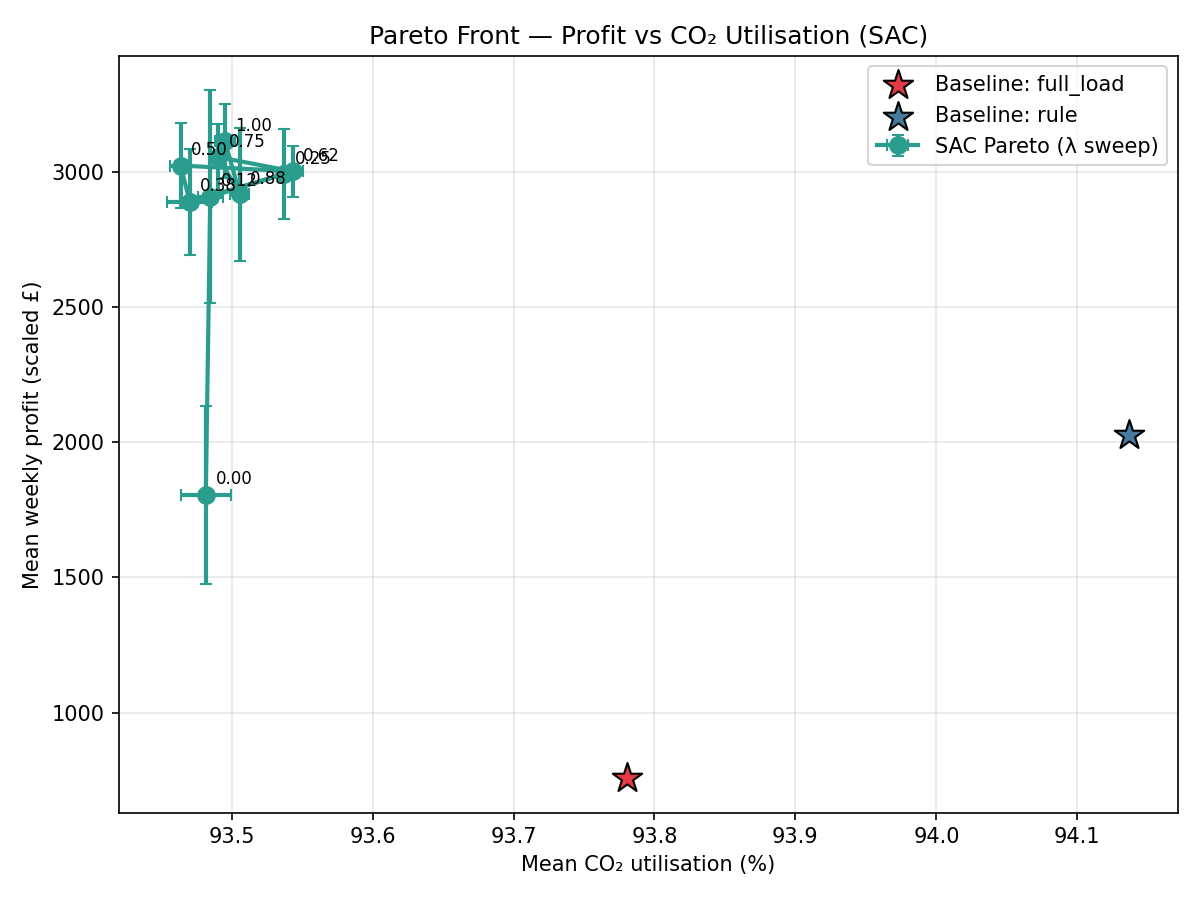
\includegraphics[width=\textwidth]{figures/fig_pareto_front.png}
    \caption{Profit vs. CO\textsubscript{2} utilisation.}
  \end{subfigure}
  \hfill
  \begin{subfigure}[t]{0.48\textwidth}
    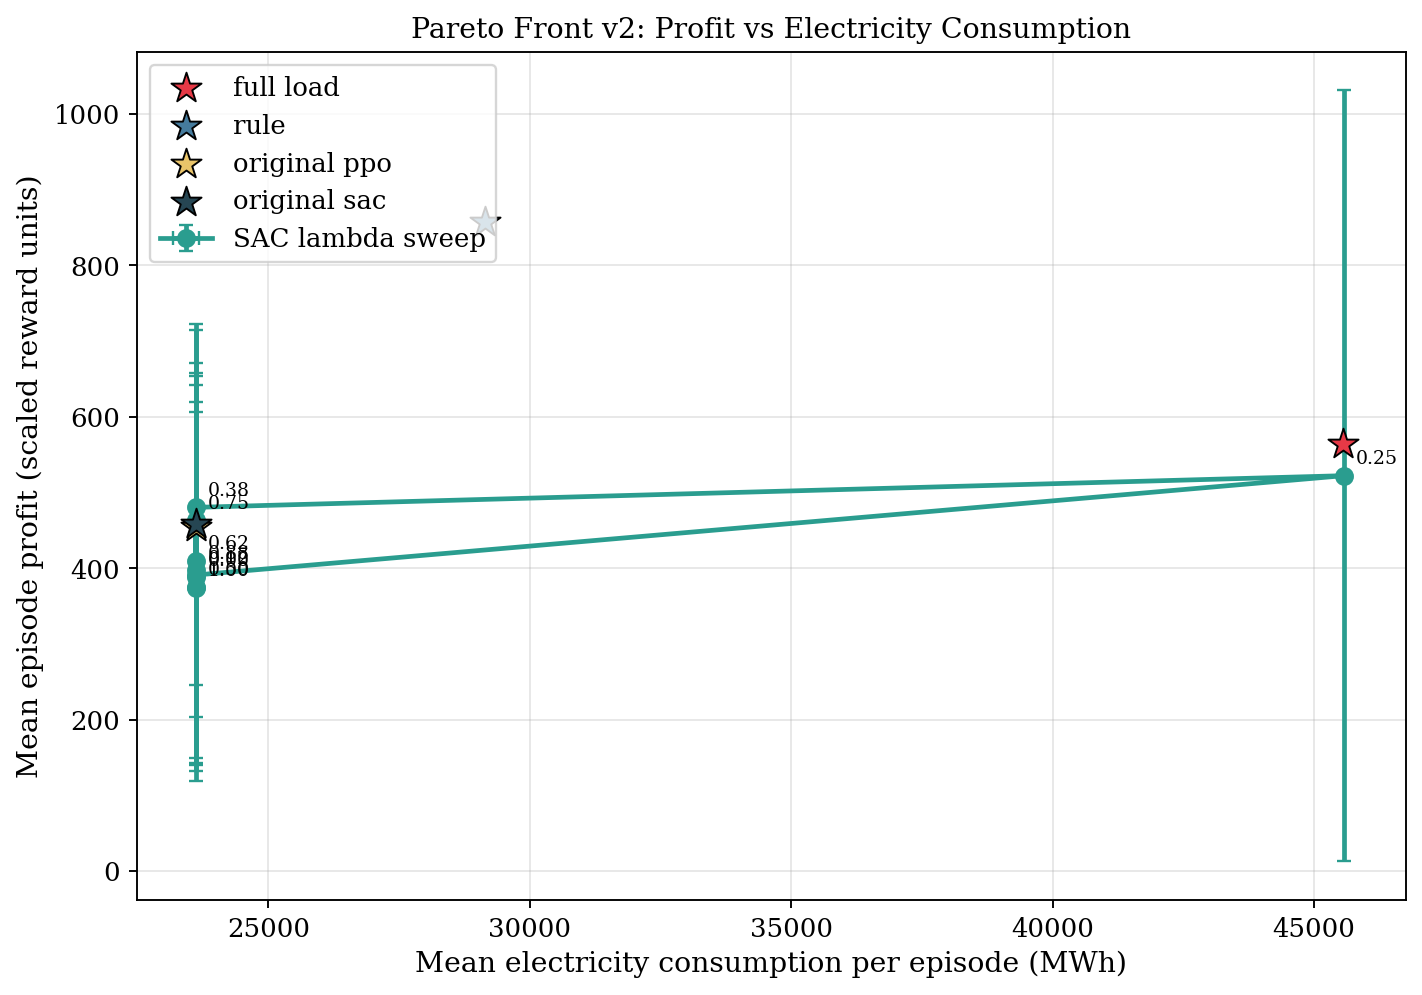
\includegraphics[width=\textwidth]{figures/fig_pareto_elec.png}
    \caption{Profit vs. electricity consumption.}
  \end{subfigure}
  \caption{Both Pareto formulations are effectively degenerate for the current
           reward structure.}
  \label{fig:pareto-negative}
\end{figure}

% ============================================================
\section{Aspen Validation Gap}
\label{sec:aspen-validation}

The remaining physical validation gap is explicit. The v2/v3 extensions are
pseudo-labelled by the simplified process model; they are not new Aspen
surfaces. To make the next validation step concrete, the repository includes
\texttt{scripts/generate\_aspen\_validation\_points.py}, which clusters the
3,360 rows of Fix~(c) step data into 20 representative operating centroids
and exports \texttt{outputs/aspen\_validation/validation\_points.csv} plus an
\texttt{aspen\_variables.txt} mapping.

\begin{table}[H]
  \centering
  \caption{Summary of the 20 Fix~(c) Aspen validation centroids. These points
           have been generated but not yet run in Aspen Plus.}
  \label{tab:aspen-centroids}
  \small
  \begin{tabular}{l rrrr}
    \toprule
    \textbf{Statistic} & \textbf{load} & \textbf{$T$ ($^\circ$C)}
      & \textbf{$P$ (bar)} & \textbf{$F_{\mathrm{H}_2}$ (kmol/hr)} \\
    \midrule
    min  & 0.02 & 253.8 & 68.8 & 57 \\
    mean & 0.15 & 275.3 & 87.7 & 403 \\
    max  & 0.45 & 278.9 & 99.2 & 1211 \\
    \bottomrule
  \end{tabular}
\end{table}

Sixteen of the twenty centroids have $F_{\mathrm{H}_2} < 800$~kmol/hr,
below the v3 lower bound. This is precisely why the 20 Aspen runs are the
next required step. They would not fully validate every possible low-load
state, but they would provide the first Aspen spot checks in the policy's
actual operating region and allow v3 predictions to be compared with physical
labels.

% ============================================================
\section{Conclusions}

\begin{enumerate}[nosep]
  \item SAC is the strongest algorithm in the tested setup. Under the
        internally consistent corrected v2 evaluation, Fix~(c) achieves
        2915.6 scaled \pounds/week on GB prices, +487\% versus full-load,
        with 0\% GPR extrapolation warnings.
  \item Cross-market transfer is promising. The GB-trained SAC retains nearly
        the same original-v1 reward on NL prices, but those transfer rewards
        should be treated as transfer evidence, not settled profit
        values.
  \item The original GPR extrapolation problem was real. Original SAC triggered
        warnings on 96.1\% of GB steps. The v2 pseudo-labelled correction
        removes the warning and preserves large RL value, but remains an
        internally consistent surrogate evaluation rather than physical
        validation.
  \item The v3 extended-$F_{\mathrm{H}_2}$ result changes the interpretation:
        scoring the v2-trained Fix~(c) policy on v3 gives
        $-161.6 \pm 6.4$. The low-load domain is economically important, so
        SAC must be retrained directly on v3 before updated economic claims
        are made.
  \item Aspen validation points have been generated but not run. The 20
        centroids are the next required physical spot checks, especially
        because 16 of 20 fall below the v3 $F_{\mathrm{H}_2}$ lower bound.
  \item The GNN is useful for edge-state prediction, not direct graph-level
        LCOM prediction. The defensible architecture is edge-state GNN plus
        scalar KPI heads and explicit economics.
  \item PPO collapse, GNN confidence penalties, and the Pareto sweeps are
        informative negative results. They support the main story by showing
        which tempting routes did not improve the current formulation.
\end{enumerate}

\end{document}
